\section{Introduction}
\begin{frame}{Introduction}
  \begin{itemize}
  \item Smart grids are becoming a necessity in order to integrate renewables, accommodate new actors, improve the observability and efficiency.
    \item The transition from conventional systems towards smart grids is challenging:
      \begin{itemize}
        \item Incorporate distributed sources of energy.
        \item Integrate storage systems.
        \item Rely less on large traditional centralized power plants.
      \end{itemize}
  \end{itemize}
  Thus, we have divided the progressive adaptations:
  \begin{table}\footnotesize
    \begin{tabular}{cc}
      \hline
      \textbf{Chapter} & \textbf{Activities} \\
      \hline
      \hline
      Phase 1 & Initial solution of the system \\
      Phase 2 & Addition of lines \\
      Phase 3 & Integration of wind and solar \\
      Phase 4 & Rehabilitated power plant and storage \\
      SGAM & HLUC related to contingencies \\
      \hline
    \end{tabular}
    \caption{Phases of the project to move towards smart grids}
  \end{table}
\end{frame}


\AtBeginSection[]
  {
     \begin{frame}<beamer>
     \frametitle{Plan}
     \tableofcontents[currentsection]
     \end{frame}
  }



\section{Phase 1}
\begin{frame}{System overview}


\begin{figure}[!htb]\centering

  \resizebox{8.0cm}{7cm}{
  \begin{circuitikz}[/tikz/circuitikz/bipoles/length=1cm, line width=0.8pt]

    % grid
    \draw[gray!50!white, line width=0.5pt] (0.0,0.0) to [short] (8.0,0.0);
    \draw[gray!50!white, line width=0.5pt] (0.0,1.6) to [short] (8.0,1.6);
    \draw[gray!50!white, line width=0.5pt] (0.0,3.2) to [short] (8.0,3.2);
    \draw[gray!50!white, line width=0.5pt] (0.0,4.8) to [short] (8.0,4.8);
    \draw[gray!50!white, line width=0.5pt] (0.0,6.4) to [short] (8.0,6.4);
    \draw[gray!50!white, line width=0.5pt] (0.0,8.0) to [short] (8.0,8.0);

    \draw[gray!50!white, line width=0.5pt] (0.0,0.0) to [short] (0.0,8.0);
    \draw[gray!50!white, line width=0.5pt] (1.6,0.0) to [short] (1.6,8.0);
    \draw[gray!50!white, line width=0.5pt] (3.2,0.0) to [short] (3.2,8.0);
    \draw[gray!50!white, line width=0.5pt] (4.8,0.0) to [short] (4.8,8.0);
    \draw[gray!50!white, line width=0.5pt] (6.4,0.0) to [short] (6.4,8.0);
    \draw[gray!50!white, line width=0.5pt] (8.0,0.0) to [short] (8.0,8.0);


    % generators
    \draw (3.2,-1.8) to [sV, fill=magenta!70!cyan] (3.2,-1.2);
    \draw [short] (3.2,-1.2) to [short] (3.2,-1.0);
    \draw (-1.8,1.6) to [sV, fill=green!50!white] (-1.2,1.6);
    \draw [short] (-1.2,1.6) to [short] (-1.0,1.6);
    \draw (9.2,1.6) to [sV, fill=cyan!50!white] (9.8,1.6);
    \draw [short] (9.2,1.6) to [short] (9.0,1.6);
    \draw (4.8,3.6) to [sV, fill=black!60!white] (4.8,3.0);
    \draw [short] (4.8,3.6) to [short] (4.8,3.8);
    \draw (8.4,4.8) to [sV, fill=yellow!60!white] (9.0,4.8);
    \draw [short] (8.0,4.8) to [short] (8.4,4.8);
    \draw (1.6,9.2) to [sV, fill=orange!60!white] (1.6,9.8);
    \draw [short] (1.6,9.0) to [short] (1.6,9.2);


    % large buses
    \draw[line width=2.5pt] (2.7,0) to [short] (3.7,0);
    \draw[line width=2.5pt] (0.0,1.1) to [short] (0,2.1);
    \draw[line width=2.5pt] (8.0,1.1) to [short] (8,2.1);
    \draw[line width=2.5pt] (1.1,8) to [short] (2.1,8);
    \draw[line width=2.5pt] (2.7,3.2) to [short] (3.7,3.2);
    \draw[line width=2.5pt] (2.7,4.8) to [short] (3.7,4.8);
    \draw[line width=2.5pt] (4.3,6.4) to [short] (5.3,6.4);
    \draw[line width=2.5pt] (0.0,5.9) to [short] (-0.0,6.9);
    \draw[line width=2.5pt] (8,4.3) to [short] (8,5.3);
    \draw[line width=2.5pt] (4.3,4.8) to [short] (5.3,4.8);

    % small buses
    \draw[line width=2.5pt] (2.9,-1) to [short] (3.5,-1);
    \draw[line width=2.5pt] (-1.0,1.3) to [short] (-1,1.9);
    \draw[line width=2.5pt] (9,1.3) to [short] (9,1.9);
    \draw[line width=2.5pt] (4.5,3.8) to [short] (5.1,3.8);
    \draw[line width=2.5pt] (1.3,9.0) to [short] (1.9,9.0);

    \draw[line width=2.5pt] (1.75,3.2) to [short] (1.75,2.6);
    \draw[line width=2.5pt] (1.75,4.8) to [short] (1.75,4.2);
    \draw[line width=2.5pt] (-0.95,6.7) to [short] (-0.95,6.1);
    \draw[line width=2.5pt] (4.5,7.35) to [short] (5.1,7.35);

    % trafos
    \draw (3.2,-1.0) to [voosource] (3.2,0.0);
    \draw (-1,1.6) to [voosource] (0,1.6);
    \draw (8,1.6) to [voosource] (9,1.6);
    \draw (1.6,8) to [voosource] (1.6,9);
    \draw (4.8,4.8) to [voosource] (4.8,3.8);

    \draw (-1,6.4) to [voosource] (0,6.4);
    \draw (4.8,6.4) to [voosource] (4.8,7.4);
    \draw (2.7,4.5) to [voosource] (1.7,4.5);
    \draw (2.7,2.9) to [voosource] (1.7,2.9);

    % loads
    \draw[-{Triangle[length=5mm, width=2mm]}, draw=blue!60!white, fill=blue!60!white] (-1,6.4) -- (-1.6,6.4);
    \draw[-{Triangle[length=5mm, width=2mm]}, draw=blue!60!white, fill=blue!60!white] (4.8,7.4) -- (4.8,8.0);
    \draw[-{Triangle[length=5mm, width=2mm]}, draw=red!60!white, fill=red!60!white] (1.7,4.5) -- (1.1,4.5);
    \draw[-{Triangle[length=5mm, width=2mm]}, draw=blue!60!white, fill=blue!60!white] (1.7,2.9) -- (1.1,2.9);

    \draw (3.0,4.8) to [short] (3.0,4.5);
    \draw (3.0,4.5) to [short] (2.7,4.5);

    \draw (3.0,3.2) to [short] (3.0,2.9);
    \draw (3.0,2.9) to [short] (2.7,2.9);

    % lines
    \draw (3.15,0) to [short] (3.15,3.2);
    \draw (3.25,0) to [short] (3.25,3.2);
    \draw (3.15,3.2) to [short] (3.15,4.8);
    \draw (3.25,3.2) to [short] (3.25,4.8);
    \draw (4.6,4.8) to [short] (4.6,5.1);
    \draw (4.6,5.1) to [short] (3.4,5.1);
    \draw (3.4,5.1) to [short] (3.4,4.8);
    \draw (3.15,4.8) to [short] (3.15,5.1);
    \draw (3.25,4.8) to [short] (3.25,5.1);
    \draw (3.15,5.1) to [short] (4.55,6.1);
    \draw (3.25,5.1) to [short] (4.65,6.1);
    \draw (4.55,6.1) to [short] (4.55,6.4);
    \draw (4.65,6.1) to [short] (4.65,6.4);
    \draw (5.0,6.4) to [short] (5.0,6.1);
    \draw (5.0,6.1) to [short] (7.7,5.1);
    \draw (7.7,5.1) to [short] (8.0,5.1);
    \draw (0,6.4) to [short] (0.3,6.4);
    \draw (0.3,6.4) to [short] (3.0,5.1);
    \draw (3.0,5.1) to [short] (3.0,4.8);


    % legend
    \draw[-{Triangle[length=5mm, width=2mm]}, draw=blue!60!white, fill=blue!60!white] (3.0,8.4) -- (4.0,8.4);
    \draw[-{Triangle[length=5mm, width=2mm]}, draw=red!60!white, fill=red!60!white] (3.0,9.1) -- (4.0,9.1);
    \draw (3.2,9.8) to [sV, fill=magenta!70!cyan] (3.8,9.8);

    \draw (6.0,9.8) to [sV, fill=black!60!white] (6.6,9.8);
    \draw (6.0,9.1) to [sV, fill=yellow!60!white] (6.6,9.1);
    \draw (6.0,8.4) to [sV, fill=green!50!white] (6.6,8.4);

    \draw (9.0,9.8) to [sV, fill=orange!60!white] (9.6,9.8);
    \draw (9.0,9.1) to [sV, fill=cyan!50!white] (9.6,9.1);

    \node at (4.73, 9.8) {\footnotesize Nuclear};
    \node at (4.66, 9.1) {\footnotesize Load I};
    \node at (4.72, 8.4) {\footnotesize Load II};

    \node at (7.64, 9.8) {\footnotesize Dismantled};
    \node at (7.49, 9.1) {\footnotesize Intercon.};
    \node at (7.28, 8.4) {\footnotesize Wind};

    \node at (10.25, 9.8) {\footnotesize Solar};
    \node at (10.40, 9.1) {\footnotesize Storage};

    \draw[gray!50!white, line width=0.5pt] (8.5,8.0) to [short] (10.1,8.0);
    \draw[gray!50!white, line width=0.5pt] (8.5,6.4) to [short] (10.1,6.4);
    \draw[gray!50!white, line width=0.5pt] (8.5,6.4) to [short] (8.5,8.0);
    \draw[gray!50!white, line width=0.5pt] (10.1,6.4) to [short] (10.1,8.0);

    \node at (9.30, 6.2) {\footnotesize 50 km};
    \node[rotate=90] at (10.3, 7.2) {\footnotesize 50 km};

    \draw [fill=gray, opacity=0.2, line width=0.01pt] (2.95,10.15) rectangle (11.0,8.05);
    \draw [fill=gray, opacity=0.2, line width=0.01pt] (11.0,8.05) rectangle (8.05,6.05);

    % buses nodes and labels
    \node at (3.6, 0.2) {8};
    \node at (3.6, -1.0) {1};
    \node at (3.6, 4.6) {9};
    \node at (1.5, 4.75) {2};
    \node at (3.6, 3.0) {10};
    \node at (1.5, 3.15) {3};
    \node at (4.4, 6.6) {11};
    \node at (4.4, 7.6) {4};
    \node at (0.2, 6.7) {12};
    \node at (-1.2, 6.7) {5};
    \node at (5.2, 4.6) {13};
    \node at (5.3, 3.8) {7};
    \node at (7.8, 4.6) {6}; 



\end{circuitikz}}

  \caption{Overview of the network}
  \label{fig:net1}
\end{figure}

\end{frame}

\subsection{Results}
\begin{frame}{Initial bus voltages}

\begin{figure}[!htb]\centering
  \resizebox{12cm}{6cm}{
\begin{tikzpicture}
    \begin{axis}[xlabel={Hour}, ylabel={$|V|$ (p.u.)}, grid=both, grid style={line width=.1pt, draw=gray!10}, major grid style={line width=.2pt,draw=gray!50}, xtick distance = 2, ytick distance = 0.02, width=12cm, height=8cm, every plot/.append style={very thick}, xmin = 1, xmax = 24, ymin=0.8, very thick, grid=both, grid style={line width=.4pt, draw=gray!10}, major grid style={line width=.8pt,draw=gray!50}, legend style={at={(1.03,0.14)},anchor=south west}]
        \addplot[color=magenta] table[col sep=comma, x=x, y=y1] {Data/phase1/ph1_vpu.csv};
        \addplot[color=red] table[col sep=comma, x=x, y=y2] {Data/phase1/ph1_vpu.csv};
        \addplot[color=green] table[col sep=comma, x=x, y=y3] {Data/phase1/ph1_vpu.csv};
        \addplot[color=cyan] table[col sep=comma, x=x, y=y4] {Data/phase1/ph1_vpu.csv};
        \addplot[color=blue] table[col sep=comma, x=x, y=y5] {Data/phase1/ph1_vpu.csv};
        \addplot[color=orange, dashed] table[col sep=comma, x=x, y=y6] {Data/phase1/ph1_vpu.csv};
        \addplot[color=magenta, dashed] table[col sep=comma, x=x, y=y8] {Data/phase1/ph1_vpu.csv};
        \addplot[color=red, dashed] table[col sep=comma, x=x, y=y9] {Data/phase1/ph1_vpu.csv};
        \addplot[color=green, dashed] table[col sep=comma, x=x, y=y10] {Data/phase1/ph1_vpu.csv};
        \addplot[color=cyan, dashed] table[col sep=comma, x=x, y=y11] {Data/phase1/ph1_vpu.csv};
        \addplot[color=blue, dashed] table[col sep=comma, x=x, y=y12] {Data/phase1/ph1_vpu.csv};
\legend{Bus 1, Bus 2, Bus 3, Bus 4, Bus 5, Bus 6, Bus 8, Bus 9, Bus 10, Bus 11, Bus 12};
\end{axis}
\end{tikzpicture}}
    \caption{Voltage profile during 24 hours for the initial grid. The low-voltage buses are plotted in solid lines; the high-voltage ones are in dashed lines.}
    \label{fig:vpu_ph1}
  \end{figure}

\end{frame}

\begin{frame}{Initial lines loading}


\begin{figure}[!htb]\centering
  \resizebox{12cm}{5.9cm}{
\begin{tikzpicture}
    \begin{axis}[xlabel={Hour}, ylabel={Load (\%)}, grid=both, grid style={line width=.1pt, draw=gray!10}, major grid style={line width=.2pt,draw=gray!50}, xtick distance = 2, ytick distance = 10, width=12cm, height=8cm, every plot/.append style={very thick}, xmin = 1, xmax = 24, ymin=0.0, very thick, grid=both, grid style={line width=.4pt, draw=gray!10}, major grid style={line width=.8pt,draw=gray!50}, legend style={at={(1.03,0.14)},anchor=south west}]
        \addplot[color=magenta] table[col sep=comma, x=x, y=l1] {Data/phase1/ph1_line.csv};
        \addplot[color=red] table[col sep=comma, x=x, y=l2] {Data/phase1/ph1_line.csv};
        \addplot[color=green] table[col sep=comma, x=x, y=l3] {Data/phase1/ph1_line.csv};
        \addplot[color=cyan] table[col sep=comma, x=x, y=l4] {Data/phase1/ph1_line.csv};
        \addplot[color=blue] table[col sep=comma, x=x, y=l5] {Data/phase1/ph1_line.csv};
\legend{Line 8-10, Line 10-9, Line 9-11, Line 9-12, Line 11-6};
\end{axis}
\end{tikzpicture}}
    \caption{Representation of the percentual loading of the lines during 24 hours}
    \label{fig:lines_ph1}
  \end{figure}

\end{frame}




\subsection{Problems identification}
\begin{frame}{Technical issues}
  The main observed issues are:

  \begin{itemize}
    \item Some load buses are below 0.9~p.u. during peak hours.
    \item While no lines surpass 100\% of load, the interconnection line is close to 90\%.
    \item In addition, the $N-1$ criteria is not met:
  \end{itemize}


\begin{table}[!htb]\centering\footnotesize
  \begin{tabular}[]{ccc}
    \hline 
    \textbf{Element} & \textbf{Disconnection time (h)} & \textbf{Consequences} \\
    \hline
    Line 8-10 & 12.50 & No load served - divergence \\
    Line 9-10 & 6.25 & No load served - divergence \\
    Line 9-11 & 8.85 & Loads at buses 2, 3 and 5 unserved \\
    Line 9-12 & 13.98 & Load at bus 5 unserved \\
    Line 11-6 & 13.98 & No load served \\
    Trafo 1-8 & 1.20 & No load served - divergence \\
    Trafo 2-9 & 1.20 & Load at bus 2 unserved \\
    Trafo 3-10 & 1.20 & Load at bus 3 unserved \\
    Trafo 4-11 & 1.20 & Load at bus 4 unserved \\
    Trafo 5-12 & 1.20 & Load at bus 5 unserved \\
    \hline
  \end{tabular}
  \caption{Disconnection time and consequences of losing each element}
  \label{tab:lt1}
\end{table}

\end{frame}


\AtBeginSection[]
  {
     \begin{frame}<beamer>
     \frametitle{Plan}
     \tableofcontents[currentsection]
     \end{frame}
  }



\section{Phase 2}
\subsection{New lines}
\begin{frame}{Potential addition of lines}


\begin{figure}[!htb]\centering

  \resizebox{8cm}{7cm}{
  \begin{circuitikz}[/tikz/circuitikz/bipoles/length=1cm, line width=0.8pt]

    % grid
    \draw[gray!50!white, line width=0.5pt] (0.0,0.0) to [short] (8.0,0.0);
    \draw[gray!50!white, line width=0.5pt] (0.0,1.6) to [short] (8.0,1.6);
    \draw[gray!50!white, line width=0.5pt] (0.0,3.2) to [short] (8.0,3.2);
    \draw[gray!50!white, line width=0.5pt] (0.0,4.8) to [short] (8.0,4.8);
    \draw[gray!50!white, line width=0.5pt] (0.0,6.4) to [short] (8.0,6.4);
    \draw[gray!50!white, line width=0.5pt] (0.0,8.0) to [short] (8.0,8.0);

    \draw[gray!50!white, line width=0.5pt] (0.0,0.0) to [short] (0.0,8.0);
    \draw[gray!50!white, line width=0.5pt] (1.6,0.0) to [short] (1.6,8.0);
    \draw[gray!50!white, line width=0.5pt] (3.2,0.0) to [short] (3.2,8.0);
    \draw[gray!50!white, line width=0.5pt] (4.8,0.0) to [short] (4.8,8.0);
    \draw[gray!50!white, line width=0.5pt] (6.4,0.0) to [short] (6.4,8.0);
    \draw[gray!50!white, line width=0.5pt] (8.0,0.0) to [short] (8.0,8.0);


    % generators
    \draw (3.2,-1.8) to [sV, fill=magenta!70!cyan] (3.2,-1.2);
    \draw [short] (3.2,-1.2) to [short] (3.2,-1.0);
    \draw (-1.8,1.6) to [sV, fill=green!50!white] (-1.2,1.6);
    \draw [short] (-1.2,1.6) to [short] (-1.0,1.6);
    \draw (9.2,1.6) to [sV, fill=cyan!50!white] (9.8,1.6);
    \draw [short] (9.2,1.6) to [short] (9.0,1.6);
    \draw (4.8,3.6) to [sV, fill=black!60!white] (4.8,3.0);
    \draw [short] (4.8,3.6) to [short] (4.8,3.8);
    \draw (8.4,4.8) to [sV, fill=yellow!60!white] (9.0,4.8);
    \draw [short] (8.0,4.8) to [short] (8.4,4.8);
    \draw (1.6,9.2) to [sV, fill=orange!60!white] (1.6,9.8);
    \draw [short] (1.6,9.0) to [short] (1.6,9.2);


    % large buses
    \draw[line width=2.5pt] (2.7,0) to [short] (3.7,0);
    \draw[line width=2.5pt] (0.0,1.1) to [short] (0,2.1);
    \draw[line width=2.5pt] (8.0,1.1) to [short] (8,2.1);
    \draw[line width=2.5pt] (1.1,8) to [short] (2.1,8);
    \draw[line width=2.5pt] (2.7,3.2) to [short] (3.7,3.2);
    \draw[line width=2.5pt] (2.7,4.8) to [short] (3.7,4.8);
    \draw[line width=2.5pt] (4.3,6.4) to [short] (5.3,6.4);
    \draw[line width=2.5pt] (0.0,5.9) to [short] (-0.0,6.9);
    \draw[line width=2.5pt] (8,4.3) to [short] (8,5.3);
    \draw[line width=2.5pt] (4.3,4.8) to [short] (5.3,4.8);

    % small buses
    \draw[line width=2.5pt] (2.9,-1) to [short] (3.5,-1);
    \draw[line width=2.5pt] (-1.0,1.3) to [short] (-1,1.9);
    \draw[line width=2.5pt] (9,1.3) to [short] (9,1.9);
    \draw[line width=2.5pt] (4.5,3.8) to [short] (5.1,3.8);
    \draw[line width=2.5pt] (1.3,9.0) to [short] (1.9,9.0);

    \draw[line width=2.5pt] (1.75,3.2) to [short] (1.75,2.6);
    \draw[line width=2.5pt] (1.75,4.8) to [short] (1.75,4.2);
    \draw[line width=2.5pt] (-0.95,6.7) to [short] (-0.95,6.1);
    \draw[line width=2.5pt] (4.5,7.35) to [short] (5.1,7.35);

    % trafos
    \draw (3.2,-1.0) to [voosource] (3.2,0.0);
    \draw (-1,1.6) to [voosource] (0,1.6);
    \draw (8,1.6) to [voosource] (9,1.6);
    \draw (1.6,8) to [voosource] (1.6,9);
    \draw (4.8,4.8) to [voosource] (4.8,3.8);

    \draw (-1,6.4) to [voosource] (0,6.4);
    \draw (4.8,6.4) to [voosource] (4.8,7.4);
    \draw (2.7,4.5) to [voosource] (1.7,4.5);
    \draw (2.7,2.9) to [voosource] (1.7,2.9);

    % loads
    \draw[-{Triangle[length=5mm, width=2mm]}, draw=blue!60!white, fill=blue!60!white] (-1,6.4) -- (-1.6,6.4);
    \draw[-{Triangle[length=5mm, width=2mm]}, draw=blue!60!white, fill=blue!60!white] (4.8,7.4) -- (4.8,8.0);
    \draw[-{Triangle[length=5mm, width=2mm]}, draw=red!60!white, fill=red!60!white] (1.7,4.5) -- (1.1,4.5);
    \draw[-{Triangle[length=5mm, width=2mm]}, draw=blue!60!white, fill=blue!60!white] (1.7,2.9) -- (1.1,2.9);

    \draw (3.0,4.8) to [short] (3.0,4.5);
    \draw (3.0,4.5) to [short] (2.7,4.5);

    \draw (3.0,3.2) to [short] (3.0,2.9);
    \draw (3.0,2.9) to [short] (2.7,2.9);

    % lines
    \draw (3.15,0) to [short] (3.15,3.2);
    \draw (3.25,0) to [short] (3.25,3.2);
    \draw (3.15,3.2) to [short] (3.15,4.8);
    \draw (3.25,3.2) to [short] (3.25,4.8);
    \draw (4.6,4.8) to [short] (4.6,5.1);
    \draw (4.6,5.1) to [short] (3.4,5.1);
    \draw (3.4,5.1) to [short] (3.4,4.8);
    \draw (3.15,4.8) to [short] (3.15,5.1);
    \draw (3.25,4.8) to [short] (3.25,5.1);
    \draw (3.15,5.1) to [short] (4.55,6.1);
    \draw (3.25,5.1) to [short] (4.65,6.1);
    \draw (4.55,6.1) to [short] (4.55,6.4);
    \draw (4.65,6.1) to [short] (4.65,6.4);
    \draw (5.0,6.4) to [short] (5.0,6.1);
    \draw (5.0,6.1) to [short] (7.7,5.1);
    \draw (7.7,5.1) to [short] (8.0,5.1);
    \draw (0,6.4) to [short] (0.3,6.4);
    \draw (0.3,6.4) to [short] (3.0,5.1);
    \draw (3.0,5.1) to [short] (3.0,4.8);

    % proposed new lines
    \draw[dashed, draw=red] (8, 4.4) to [short] (3.5,4.4);
    \draw[dashed, draw=red] (3.5,4.4) to [short] (3.5,4.8);
    \draw[dashed, draw=red] (8,4.4) to [short] (3.5,3.2);
    \draw[dashed, draw=red] (4.5,6.4) to [short] (0,6.4);
    \draw[dashed, draw=red] (3,0) to [short] (3,4.8);
    \draw[dashed, draw=red] (3,3.2) to [short] (0,6.2);
    \draw[dashed, draw=red] (3,0) to [short] (0,6.2);

    \draw[dashed, draw=red] (8,5.0) to [short] (4.8,5.0);
    \draw[dashed, draw=red] (4.8,5.0) to [short] (4.8,4.8);
    \draw[dashed, draw=red] (8,4.4) to [short] (3.3,0);

    \draw[draw=red] (6,4.85) to [short] (6.3,5.15);
    \draw[draw=red] (6.2,4.85) to [short] (6.5,5.15);

    \draw[draw=red] (6,4.25) to [short] (6.3,4.55);
    \draw[draw=red] (6.2,4.25) to [short] (6.5,4.55);

    \draw[draw=red] (2,6.25) to [short] (2.3,6.55);
    \draw[draw=red] (2.2,6.25) to [short] (2.5,6.55);

    \draw[draw=red] (2.85,1.5) to [short] (3.15,1.8);
    \draw[draw=red] (2.85,1.7) to [short] (3.15,2.0);

    \draw[draw=red] (2.3,3.6) to [short] (2.6,3.9);
    \draw[draw=red] (2.2,3.7) to [short] (2.5,4.0);

    \draw[draw=red] (5.3,1.6) to [short] (5.0,1.9);
    \draw[draw=red] (5.4,1.7) to [short] (5.1,2.0);

    % legend
    \draw[-{Triangle[length=5mm, width=2mm]}, draw=blue!60!white, fill=blue!60!white] (3.0,8.4) -- (4.0,8.4);
    \draw[-{Triangle[length=5mm, width=2mm]}, draw=red!60!white, fill=red!60!white] (3.0,9.1) -- (4.0,9.1);
    \draw (3.2,9.8) to [sV, fill=magenta!70!cyan] (3.8,9.8);

    \draw (6.0,9.8) to [sV, fill=black!60!white] (6.6,9.8);
    \draw (6.0,9.1) to [sV, fill=yellow!60!white] (6.6,9.1);
    \draw (6.0,8.4) to [sV, fill=green!50!white] (6.6,8.4);

    \draw (9.0,9.8) to [sV, fill=orange!60!white] (9.6,9.8);
    \draw (9.0,9.1) to [sV, fill=cyan!50!white] (9.6,9.1);
    \draw[dashed, draw=red] (9.0,8.4) to [short] (9.5,8.4);

    \node at (4.73, 9.8) {\footnotesize Nuclear};
    \node at (4.66, 9.1) {\footnotesize Load I};
    \node at (4.72, 8.4) {\footnotesize Load II};

    \node at (7.64, 9.8) {\footnotesize Dismantled};
    \node at (7.49, 9.1) {\footnotesize Intercon.};
    \node at (7.28, 8.4) {\footnotesize Wind};

    \node at (10.25, 9.8) {\footnotesize Solar};
    \node at (10.40, 9.1) {\footnotesize Storage};
    \node at (10.45, 8.4) {\footnotesize New line};

    \draw[gray!50!white, line width=0.5pt] (8.5,8.0) to [short] (10.1,8.0);
    \draw[gray!50!white, line width=0.5pt] (8.5,6.4) to [short] (10.1,6.4);
    \draw[gray!50!white, line width=0.5pt] (8.5,6.4) to [short] (8.5,8.0);
    \draw[gray!50!white, line width=0.5pt] (10.1,6.4) to [short] (10.1,8.0);

    \node at (9.30, 6.2) {\footnotesize 50 km};
    \node[rotate=90] at (10.3, 7.2) {\footnotesize 50 km};

    \draw [fill=gray, opacity=0.2, line width=0.01pt] (2.95,10.15) rectangle (11.5,8.05);
    \draw [fill=gray, opacity=0.2, line width=0.01pt] (11.5,8.05) rectangle (8.05,6.05);

    % buses nodes and labels
    \node at (3.6, 0.2) {8};
    \node at (3.6, -1.0) {1};
    \node at (3.6, 4.6) {9};
    \node at (1.75, 5.0) {2};
    \node at (3.6, 3.0) {10};
    \node at (1.75, 3.45) {3};
    \node at (4.4, 6.6) {11};
    \node at (4.4, 7.6) {4};
    \node at (0.2, 6.7) {12};
    \node at (-1.2, 6.7) {5};
    \node at (5.2, 4.6) {13};
    \node at (5.3, 3.8) {7};
    \node at (7.8, 4.6) {6}; 

\end{circuitikz}}

  \caption{Overview of the new network. Double line indicates double circuit.}
  \label{fig:net2}
\end{figure}

\end{frame}


\subsection{Contingency analysis}
\begin{frame}{Algorithm to compute contingencies}

\begin{algorithm}[H]
\DontPrintSemicolon
  
% \KwInput{\texttt{net} initialized class, $j$, $n$}
  % \KwOutput{stored results}

  \textbf{Input:} \texttt{net} initialized class, $j$, $n$

  \textbf{Output:} stored results

  Generate permutations $\forall \bm{\sigma}_{g}$ where $g=[1,2,...,2^{(n-j)}]$

  \For{$i=[1,2,...,j]$}
  {
    $\sigma_i\gets$\texttt{false}

    $\sigma_r\gets$\texttt{true}, where $r\neq i$ and $r\leq j$

    $\mathcal{A}\gets \{\mathbf{1}_{\sigma_{1}}, \mathbf{1}_{\sigma_{2}},..., \mathbf{1}_{\sigma_{j}}\}$\\

    \For{$g=[1,2,...,2^{(n-j)}]$}
    {
      $[\sigma_{j+1}, \sigma_{j+2},..., \sigma_n] \gets \bm{\sigma}_g$

    $\mathcal{B} \gets \{\mathbf{1}_{\sigma_{j+1}}, \mathbf{1}_{\sigma_{j+2}},..., \mathbf{1}_{\sigma_{n}}\}$\\

    $\mathcal{N} \gets \mathcal{A} \cup \mathcal{B}$

    \texttt{pandapower.timeseries.run\_timeseries(}$\mathcal{N}$,\texttt{net)}

    Store results
    }
  }
\caption{Pseudocode to solve the contingencies}
\label{alg:1}
\end{algorithm}

\end{frame}


\subsection{Results}

\begin{frame}{Contingency analysis for additional lines}
Top 10 optimal configurations. Requirements are met and cost is minimized.

\begin{table}[!htb]\centering\footnotesize
  \begin{tabular}{ccc}
    \hline
    \textbf{Identifier} & \textbf{New lines} & \textbf{Infraestructure cost (M\texteuro)}\\
    \hline
    19 & [6-13, 6-10, 8-9, 10-12] &  359.50 \\
    214 & [6-13, 6-10, 11-12, 8-9] & 362.99 \\
    77 & [6-13, 8-9, 10-12, 9-6] & 375.04 \\
    49 & [6-13, 11-12, 8-9, 9-6] & 378.54 \\
    80 & [6-13, 6-10, 11-12, 8-9, 10-12] & 420.63 \\
    189 & [6-13, 6-10, 8-9, 10-12, 9-6] & 420.63 \\
    45 & [6-13, 6-10, 8-9, 10-12, 8-12] & 423.96 \\
    70 & [6-13, 8-9, 10-12, 9-6] & 424.12 \\
    157 & [6-13, 6-10, 11-12, 8-9, 8-12] & 427.46 \\
    250 & [6-13, 11-12, 8-9, 10-12, 9-6] & 436.17 \\
    \hline
  \end{tabular}
  \caption{Best configurations with the additional lines}
  \label{tab:top10_1}
\end{table}

Serious need to install more lines connected to the interconnection bus.
\end{frame}

\begin{frame}{Contingency analysis for a voltage level of 400~kV}
  Same for a rise in the voltage.

\begin{table}[!htb]\footnotesize
    \centering
    \begin{tabular}{ccccc}
    \hline
    \textbf{Identifier} & \textbf{New lines} & \textbf{Lines (M\texteuro)} & \textbf{Transformers (M\texteuro)} & \textbf{Total (M\texteuro)} \\
        \hline
    163 & [6-13, 8-9, 10-12] & 313.92 & 64.79 & 378.71 \\
    133 & [6-13, 11-12, 8-9] & 317.41 & 64.79 & 382.20 \\
    235 & [6-13, 8-9, 8-12] & 320.75 & 64.79 & 385.54 \\
    30 & [6-13, 8-12, 6-8] & 346.07 & 64.79 & 410.86 \\
    19 & [6-13, 6-10, 8-9, 10-12] & 359.50 & 64.79 & 424.29 \\
    214 & [6-13, 6-10, 11-12, 8-9] & 362.99 & 64.79 & 427.78 \\
    58 & [6-13, 6-10, 8-9, 8-12] & 366.33 & 64.79 & 431.12 \\
    77 & [6-13, 8-9, 10-12, 9-6] & 375.04 & 64.79 & 439.83 \\
    169 & [6-13, 8-9, 10-12, 8-12] & 378.38 & 64.79 & 443.17 \\
    49 & [6-13, 11-12, 8-9, 9-6] & 378.54 & 64.79 & 443.33 \\
        \hline
    \end{tabular}
    \caption{Economic results of replacing the substations}
    \label{tab:cost_trafos2}
\end{table}
Three additional lines instead of four are required. However, the cost becomes a bit larger. It becomes a sub-optimal choice.

\end{frame}

\AtBeginSection[]
  {
     \begin{frame}<beamer>
     \frametitle{Plan}
     \tableofcontents[currentsection]
     \end{frame}
  }

\section{Phase 3}
\subsection{Placement of renewables}
\begin{frame}{Connection of renewables to the system}


\begin{figure}[!htb]\centering

  \resizebox{8cm}{7cm}{
  \begin{circuitikz}[/tikz/circuitikz/bipoles/length=1cm, line width=0.8pt]

    % grid
    \draw[gray!50!white, line width=0.5pt] (0.0,0.0) to [short] (8.0,0.0);
    \draw[gray!50!white, line width=0.5pt] (0.0,1.6) to [short] (8.0,1.6);
    \draw[gray!50!white, line width=0.5pt] (0.0,3.2) to [short] (8.0,3.2);
    \draw[gray!50!white, line width=0.5pt] (0.0,4.8) to [short] (8.0,4.8);
    \draw[gray!50!white, line width=0.5pt] (0.0,6.4) to [short] (8.0,6.4);
    \draw[gray!50!white, line width=0.5pt] (0.0,8.0) to [short] (8.0,8.0);

    \draw[gray!50!white, line width=0.5pt] (0.0,0.0) to [short] (0.0,8.0);
    \draw[gray!50!white, line width=0.5pt] (1.6,0.0) to [short] (1.6,8.0);
    \draw[gray!50!white, line width=0.5pt] (3.2,0.0) to [short] (3.2,8.0);
    \draw[gray!50!white, line width=0.5pt] (4.8,0.0) to [short] (4.8,8.0);
    \draw[gray!50!white, line width=0.5pt] (6.4,0.0) to [short] (6.4,8.0);
    \draw[gray!50!white, line width=0.5pt] (8.0,0.0) to [short] (8.0,8.0);


    % generators
    \draw (3.2,-1.8) to [sV, fill=magenta!70!cyan] (3.2,-1.2);
    \draw [short] (3.2,-1.2) to [short] (3.2,-1.0);
    \draw (-1.8,1.6) to [sV, fill=green!50!white] (-1.2,1.6);
    \draw [short] (-1.2,1.6) to [short] (-1.0,1.6);
    \draw (9.2,1.6) to [sV, fill=cyan!50!white] (9.8,1.6);
    \draw [short] (9.2,1.6) to [short] (9.0,1.6);
    \draw (4.8,3.6) to [sV, fill=black!60!white] (4.8,3.0);
    \draw [short] (4.8,3.6) to [short] (4.8,3.8);
    \draw (8.4,4.8) to [sV, fill=yellow!60!white] (9.0,4.8);
    \draw [short] (8.0,4.8) to [short] (8.4,4.8);
    \draw (1.6,9.2) to [sV, fill=orange!60!white] (1.6,9.8);
    \draw [short] (1.6,9.0) to [short] (1.6,9.2);


    % large buses
    \draw[line width=2.5pt] (2.7,0) to [short] (3.7,0);
    \draw[line width=2.5pt] (0.0,1.1) to [short] (0,2.1);
    \draw[line width=2.5pt] (8.0,1.1) to [short] (8,2.1);
    \draw[line width=2.5pt] (1.1,8) to [short] (2.1,8);
    \draw[line width=2.5pt] (2.7,3.2) to [short] (3.7,3.2);
    \draw[line width=2.5pt] (2.7,4.8) to [short] (3.7,4.8);
    \draw[line width=2.5pt] (4.3,6.4) to [short] (5.3,6.4);
    \draw[line width=2.5pt] (0.0,5.9) to [short] (-0.0,6.9);
    \draw[line width=2.5pt] (8,4.3) to [short] (8,5.3);
    \draw[line width=2.5pt] (4.3,4.8) to [short] (5.3,4.8);

    % small buses
    \draw[line width=2.5pt] (2.9,-1) to [short] (3.5,-1);
    \draw[line width=2.5pt] (-1.0,1.3) to [short] (-1,1.9);
    \draw[line width=2.5pt] (9,1.3) to [short] (9,1.9);
    \draw[line width=2.5pt] (4.5,3.8) to [short] (5.1,3.8);
    \draw[line width=2.5pt] (1.3,9.0) to [short] (1.9,9.0);

    \draw[line width=2.5pt] (1.75,3.2) to [short] (1.75,2.6);
    \draw[line width=2.5pt] (1.75,4.8) to [short] (1.75,4.2);
    \draw[line width=2.5pt] (-0.95,6.7) to [short] (-0.95,6.1);
    \draw[line width=2.5pt] (4.5,7.35) to [short] (5.1,7.35);

    % trafos
    \draw (3.2,-1.0) to [voosource] (3.2,0.0);
    \draw (-1,1.6) to [voosource] (0,1.6);
    \draw (8,1.6) to [voosource] (9,1.6);
    \draw (1.6,8) to [voosource] (1.6,9);
    \draw (4.8,4.8) to [voosource] (4.8,3.8);

    \draw (-1,6.4) to [voosource] (0,6.4);
    \draw (4.8,6.4) to [voosource] (4.8,7.4);
    \draw (2.7,4.5) to [voosource] (1.7,4.5);
    \draw (2.7,2.9) to [voosource] (1.7,2.9);

    % loads
    \draw[-{Triangle[length=5mm, width=2mm]}, draw=blue!60!white, fill=blue!60!white] (-1,6.4) -- (-1.6,6.4);
    \draw[-{Triangle[length=5mm, width=2mm]}, draw=blue!60!white, fill=blue!60!white] (4.8,7.4) -- (4.8,8.0);
    \draw[-{Triangle[length=5mm, width=2mm]}, draw=red!60!white, fill=red!60!white] (1.7,4.5) -- (1.1,4.5);
    \draw[-{Triangle[length=5mm, width=2mm]}, draw=blue!60!white, fill=blue!60!white] (1.7,2.9) -- (1.1,2.9);

    \draw (3.0,4.8) to [short] (3.0,4.5);
    \draw (3.0,4.5) to [short] (2.7,4.5);

    \draw (2.75,3.2) to [short] (2.75,2.9);
    \draw (2.75,2.9) to [short] (2.7,2.9);

    % lines
    \draw (3.15,0) to [short] (3.15,3.2);
    \draw (3.25,0) to [short] (3.25,3.2);
    \draw (3.15,3.2) to [short] (3.15,4.8);
    \draw (3.25,3.2) to [short] (3.25,4.8);
    \draw (4.6,4.8) to [short] (4.6,5.1);
    \draw (4.6,5.1) to [short] (3.4,5.1);
    \draw (3.4,5.1) to [short] (3.4,4.8);
    \draw (3.15,4.8) to [short] (3.15,5.1);
    \draw (3.25,4.8) to [short] (3.25,5.1);
    \draw (3.15,5.1) to [short] (4.55,6.1);
    \draw (3.25,5.1) to [short] (4.65,6.1);
    \draw (4.55,6.1) to [short] (4.55,6.4);
    \draw (4.65,6.1) to [short] (4.65,6.4);
    \draw (5.0,6.4) to [short] (5.0,6.1);
    \draw (5.0,6.1) to [short] (7.7,5.1);
    \draw (7.7,5.1) to [short] (8.0,5.1);
    \draw (0,6.4) to [short] (0.3,6.4);
    \draw (0.3,6.4) to [short] (3.0,5.1);
    \draw (3.0,5.1) to [short] (3.0,4.8);


    % proposed new lines
    \draw[dashed, draw=red] (8, 4.4) to [short] (3.5,4.4);
    \draw[dashed, draw=red] (3.5,4.4) to [short] (3.5,4.8);
    % \draw[dashed, draw=red] (8,4.4) to [short] (3.5,3.2);
    \draw[dashed, draw=red] (4.5,6.4) to [short] (0,6.4);
    \draw[dashed, draw=red] (3,0) to [short] (3,4.8);
    \draw[dashed, draw=red] (3,3.2) to [short] (0,6.2);
    \draw[dashed, draw=red] (3,0) to [short] (0,6.2);

    % \draw[dashed, draw=red] (8,5.0) to [short] (4.8,5.0);
    % \draw[dashed, draw=red] (4.8,5.0) to [short] (4.8,4.8);
    \draw[dashed, draw=red] (8,4.4) to [short] (3.3,0);

    \draw[draw=red] (6.0,4.25) to [short] (6.3,4.55);
    \draw[draw=red] (6.2,4.25) to [short] (6.5,4.55);

    % \draw[draw=red] (6,4.85) to [short] (6.3,5.15);
    % \draw[draw=red] (6.2,4.85) to [short] (6.5,5.15);

    % \draw[draw=red] (6,4.25) to [short] (6.3,4.55);
    % \draw[draw=red] (6.2,4.25) to [short] (6.5,4.55);

    \draw[draw=red] (2,6.25) to [short] (2.3,6.55);
    \draw[draw=red] (2.2,6.25) to [short] (2.5,6.55);

    \draw[draw=red] (2.85,1.5) to [short] (3.15,1.8);
    \draw[draw=red] (2.85,1.7) to [short] (3.15,2.0);

    \draw[draw=red] (2.3,3.6) to [short] (2.6,3.9);
    \draw[draw=red] (2.2,3.7) to [short] (2.5,4.0);

    \draw[draw=red] (5.3,1.6) to [short] (5.0,1.9);
    \draw[draw=red] (5.4,1.7) to [short] (5.1,2.0);

    % lines for rene and solid interconnection
    \draw (0,6.7) to [short] (0.3,6.7);
    \draw (0,6.8) to [short] (0.3,6.8);
    \draw (0.3,6.7) to [short] (1.65,7.7);
    \draw (0.3,6.8) to [short] (1.55,7.7);
    \draw (1.65,7.7) to [short] (1.65,8.0);
    \draw (1.55,7.7) to [short] (1.55,8.0);

    \draw (0,1.55) to [short] (2.85,1.55);
    \draw (0,1.65) to [short] (2.75,1.65);
    \draw (2.85,1.55) to [short] (2.85,3.2);
    \draw (2.75,1.65) to [short] (2.75,3.2);

    \draw (8,4.9) to [short] (4.9, 4.9);
    \draw (8,5.0) to [short] (4.8, 5.0);
    \draw (4.9,4.9) to [short] (4.9,4.8);
    \draw (4.8,5.0) to [short] (4.8,4.8);

    \draw (8.0,4.4) to [short] (7.7,4.4);
    \draw (7.7,4.4) to [short] (3.5,3.5);
    \draw (3.5,3.5) to [short] (3.5,3.2);

    % legend
    \draw[-{Triangle[length=5mm, width=2mm]}, draw=blue!60!white, fill=blue!60!white] (3.0,8.4) -- (4.0,8.4);
    \draw[-{Triangle[length=5mm, width=2mm]}, draw=red!60!white, fill=red!60!white] (3.0,9.1) -- (4.0,9.1);
    \draw (3.2,9.8) to [sV, fill=magenta!70!cyan] (3.8,9.8);

    \draw (6.0,9.8) to [sV, fill=black!60!white] (6.6,9.8);
    \draw (6.0,9.1) to [sV, fill=yellow!60!white] (6.6,9.1);
    \draw (6.0,8.4) to [sV, fill=green!50!white] (6.6,8.4);

    \draw (9.0,9.8) to [sV, fill=orange!60!white] (9.6,9.8);
    \draw (9.0,9.1) to [sV, fill=cyan!50!white] (9.6,9.1);
    \draw[dashed, draw=red] (9.0,8.4) to [short] (9.5,8.4);

    \node at (4.73, 9.8) {\footnotesize Nuclear};
    \node at (4.66, 9.1) {\footnotesize Load I};
    \node at (4.72, 8.4) {\footnotesize Load II};

    \node at (7.64, 9.8) {\footnotesize Dismantled};
    \node at (7.49, 9.1) {\footnotesize Intercon.};
    \node at (7.28, 8.4) {\footnotesize Wind};

    \node at (10.25, 9.8) {\footnotesize Solar};
    \node at (10.40, 9.1) {\footnotesize Storage};
    \node at (10.45, 8.4) {\footnotesize New line};

    \draw[gray!50!white, line width=0.5pt] (8.5,8.0) to [short] (10.1,8.0);
    \draw[gray!50!white, line width=0.5pt] (8.5,6.4) to [short] (10.1,6.4);
    \draw[gray!50!white, line width=0.5pt] (8.5,6.4) to [short] (8.5,8.0);
    \draw[gray!50!white, line width=0.5pt] (10.1,6.4) to [short] (10.1,8.0);

    \node at (9.30, 6.2) {\footnotesize 50 km};
    \node[rotate=90] at (10.3, 7.2) {\footnotesize 50 km};

    \draw [fill=gray, opacity=0.2, line width=0.01pt] (2.95,10.15) rectangle (11.5,8.05);
    \draw [fill=gray, opacity=0.2, line width=0.01pt] (11.5,8.05) rectangle (8.05,6.05);

    % buses nodes and labels
    \node at (3.6, 0.2) {8};
    \node at (3.6, -1.0) {1};
    \node at (3.6, 4.6) {9};
    \node at (1.75, 5.0) {2};
    \node at (3.6, 3.0) {10};
    \node at (1.75, 3.45) {3};
    \node at (4.4, 6.6) {11};
    \node at (4.4, 7.6) {4};
    \node at (0.0, 7.1) {12};
    \node at (-1.2, 6.7) {5};
    \node at (5.2, 4.6) {13};
    \node at (5.3, 3.7) {7};
    \node at (7.8, 4.6) {6}; 

    \node at (0.9, 8.0) {15};
    \node at (1.1, 9.0) {14};

    \node at (0.0, 0.9) {16};
    \node at (-1.0, 1.1) {17};
    % \node at (1.3, 8.0) {14};

\end{circuitikz}}

  \caption{Overview of the network with renewables and the potential addition of lines}
  \label{fig:netrene}
\end{figure}
\end{frame}

\begin{frame}{Solar resources}
  Profile extracted from PVGIS:
\begin{figure}[!htb]\centering
  \resizebox{12cm}{5cm}{
\begin{tikzpicture}
    \begin{axis}[xlabel={Hour}, ylabel={$G$ (W/m$^2$)}, axis y line*=right, grid=both, grid style={line width=.1pt, draw=gray!10}, major grid style={line width=.2pt,draw=gray!50}, xtick distance = 2, ytick distance = 100, width=12cm, height=6cm, every plot/.append style={very thick}, xmin = 1, xmax = 23, ymin=0.0, ymax=900, very thick, grid=both, grid style={line width=.4pt, draw=gray!10}, major grid style={line width=.8pt,draw=gray!50}, legend style={at={(0.8,0.1)},anchor=south west}]
        \addplot[color=orange] table[col sep=comma, x=x, y=y] {Data/phase3/G.csv};
        \legend{$G$}
\end{axis}

    \begin{axis}[xlabel={Hour}, hide x axis, ylabel={$P$ (MW)}, axis y line*=left,  xtick distance = 2, ytick distance = 10, width=12cm, height=6cm, every plot/.append style={very thick}, xmin = 1, xmax = 24, ymin=0.0, ymax = 96, very thick, legend style={at={(0.8,0.25)},anchor=south west}]
        \addplot[color=red] table[col sep=comma, x=x, y=y] {Data/phase3/Ppv.csv};
        \legend{$P$}
\end{axis}

\end{tikzpicture}}
\caption{Irradiance and power from the PV plant along a representative day}
    \label{fig:pvpx}
  \end{figure}

\end{frame}


\begin{frame}{Wind resources}
Profile extracted from NASA database:

\begin{figure}[!htb]\centering
  \resizebox{12cm}{5cm}{
\begin{tikzpicture}
    \begin{axis}[xlabel={Hour}, ylabel={$v_w$ (m/s)}, axis y line*=right, grid=both, grid style={line width=.1pt, draw=gray!10}, major grid style={line width=.2pt,draw=gray!50}, xtick distance = 2, ytick distance = 1, width=12cm, height=6cm, every plot/.append style={very thick}, xmin = 1, xmax = 23, ymin=0.0, ymax=12, very thick, grid=both, grid style={line width=.4pt, draw=gray!10}, major grid style={line width=.8pt,draw=gray!50}, legend style={at={(0.8,0.1)},anchor=south west}]
        \addplot[color=orange] table[col sep=comma, x=x, y=y] {Data/phase3/vw.csv};
        \legend{$v_w$};
\end{axis}

    \begin{axis}[xlabel={Hour}, hide x axis, ylabel={$P$ (MW)}, axis y line*=left,  xtick distance = 2, ytick distance = 1, width=12cm, height=6cm, every plot/.append style={very thick}, xmin = 1, xmax = 24, ymin=0.0, ymax = 10, very thick, legend style={at={(0.8,0.25)},anchor=south west}]
        \addplot[color=red] table[col sep=comma, x=x, y=y] {Data/phase3/Pwind.csv};
        \legend{$P$};
\end{axis}
\end{tikzpicture}}
\caption{Wind speed and output power from the wind farm}
    \label{fig:windx}
  \end{figure}

\end{frame}


\subsection{Results}
\begin{frame}{Improvement due to renewables}
  It is worth it to compare the variation of the magnitudes due to renewables in normal operation.

\begin{table}[!htb]\centering\footnotesize
  \begin{tabular}{lrr}
    \hline
    \textbf{Attributes} & \textbf{Without renewables} & \textbf{With renewables}\\
    \hline
    $V_{min}$ (p.u.) & 0.962 & 0.968 \\
    $V_{max}$ (p.u.) & 1.050 & 1.050 \\
    Max. load (\%) & 41.65 & 40.76 \\
    Max. losses (MW) & 14.54 & 14.43 \\
    Correct operation? & Yes & Yes \\
    \hline
  \end{tabular}
  \caption{Main results to compare between the grid with and without renewables}
  \label{tab:compare}
\end{table}
Results improve a bit. Unfortunately, the installed renewable power is not significant to cause a large impact.

\end{frame}

\begin{frame}{Contingency analysis}
  Still four lines have to be added (interconnection lines have been set as static). The cost increases slightly because renewable power plants require extra lines.
\begin{table}[!htb]\centering\footnotesize
  \begin{tabular}{ccc}
    \hline
    \textbf{Identifier} & \textbf{New lines} & \textbf{Infraestructure cost (M\texteuro)}\\
    \hline
    24 & [8-9, 10-12] & 402.71 \\
    12 & [8-9, 9-6] & 406.21 \\
    46 & [11-12, 8-9] & 406.21 \\
    8 & [8-9, 8-12] & 409.54 \\
    0 & [11-12, 8-9, 10-12] & 463.84 \\
    4 & [8-9, 10-12, 9-6] & 463.84 \\
    37 & [11-12, 10-12, 9-6] & 463.84 \\
    63 & [8-9, 10-12, 8-12] & 467.18 \\
    20 & [11-12, 8-9, 9-6] & 467.34 \\
    38 & [11-12, 8-9, 8-12] & 470.67 \\
    \hline
  \end{tabular}
  \caption{Best configurations with the additional lines}
  \label{tab:top10_rene}
\end{table}

\end{frame}



\AtBeginSection[]
  {
     \begin{frame}<beamer>
     \frametitle{Plan}
     \tableofcontents[currentsection]
     \end{frame}
  }


  \section{Phase 4}
  \subsection{Storage + power plant}
  \begin{frame}{Connection of a storage unit and a dismantled plant}


\begin{figure}[!htb]\centering

  \resizebox{8cm}{7cm}{
  \begin{circuitikz}[/tikz/circuitikz/bipoles/length=1cm, line width=0.8pt]

    % grid
    \draw[gray!50!white, line width=0.5pt] (0.0,0.0) to [short] (8.0,0.0);
    \draw[gray!50!white, line width=0.5pt] (0.0,1.6) to [short] (8.0,1.6);
    \draw[gray!50!white, line width=0.5pt] (0.0,3.2) to [short] (8.0,3.2);
    \draw[gray!50!white, line width=0.5pt] (0.0,4.8) to [short] (8.0,4.8);
    \draw[gray!50!white, line width=0.5pt] (0.0,6.4) to [short] (8.0,6.4);
    \draw[gray!50!white, line width=0.5pt] (0.0,8.0) to [short] (8.0,8.0);

    \draw[gray!50!white, line width=0.5pt] (0.0,0.0) to [short] (0.0,8.0);
    \draw[gray!50!white, line width=0.5pt] (1.6,0.0) to [short] (1.6,8.0);
    \draw[gray!50!white, line width=0.5pt] (3.2,0.0) to [short] (3.2,8.0);
    \draw[gray!50!white, line width=0.5pt] (4.8,0.0) to [short] (4.8,8.0);
    \draw[gray!50!white, line width=0.5pt] (6.4,0.0) to [short] (6.4,8.0);
    \draw[gray!50!white, line width=0.5pt] (8.0,0.0) to [short] (8.0,8.0);


    % generators
    \draw (3.2,-1.8) to [sV, fill=magenta!70!cyan] (3.2,-1.2);
    \draw [short] (3.2,-1.2) to [short] (3.2,-1.0);
    \draw (-1.8,1.6) to [sV, fill=green!50!white] (-1.2,1.6);
    \draw [short] (-1.2,1.6) to [short] (-1.0,1.6);
    \draw (9.2,1.6) to [sV, fill=cyan!50!white] (9.8,1.6);
    \draw [short] (9.2,1.6) to [short] (9.0,1.6);
    \draw (4.8,3.6) to [sV, fill=black!60!white] (4.8,3.0);
    \draw [short] (4.8,3.6) to [short] (4.8,3.8);
    \draw (8.4,4.8) to [sV, fill=yellow!60!white] (9.0,4.8);
    \draw [short] (8.0,4.8) to [short] (8.4,4.8);
    \draw (1.6,9.2) to [sV, fill=orange!60!white] (1.6,9.8);
    \draw [short] (1.6,9.0) to [short] (1.6,9.2);


    % large buses
    \draw[line width=2.5pt] (2.7,0) to [short] (3.7,0);
    \draw[line width=2.5pt] (0.0,1.1) to [short] (0,2.1);
    \draw[line width=2.5pt] (8.0,1.1) to [short] (8,2.1);
    \draw[line width=2.5pt] (1.1,8) to [short] (2.1,8);
    \draw[line width=2.5pt] (2.7,3.2) to [short] (3.7,3.2);
    \draw[line width=2.5pt] (2.7,4.8) to [short] (3.7,4.8);
    \draw[line width=2.5pt] (4.3,6.4) to [short] (5.3,6.4);
    \draw[line width=2.5pt] (0.0,5.9) to [short] (-0.0,6.9);
    \draw[line width=2.5pt] (8,4.3) to [short] (8,5.3);
    \draw[line width=2.5pt] (4.3,4.8) to [short] (5.3,4.8);

    % small buses
    \draw[line width=2.5pt] (2.9,-1) to [short] (3.5,-1);
    \draw[line width=2.5pt] (-1.0,1.3) to [short] (-1,1.9);
    \draw[line width=2.5pt] (9,1.3) to [short] (9,1.9);
    \draw[line width=2.5pt] (4.5,3.8) to [short] (5.1,3.8);
    \draw[line width=2.5pt] (1.3,9.0) to [short] (1.9,9.0);

    \draw[line width=2.5pt] (1.75,3.2) to [short] (1.75,2.6);
    \draw[line width=2.5pt] (1.75,4.8) to [short] (1.75,4.2);
    \draw[line width=2.5pt] (-0.95,6.7) to [short] (-0.95,6.1);
    \draw[line width=2.5pt] (4.5,7.35) to [short] (5.1,7.35);

    % trafos
    \draw (3.2,-1.0) to [voosource] (3.2,0.0);
    \draw (-1,1.6) to [voosource] (0,1.6);
    \draw (8,1.6) to [voosource] (9,1.6);
    \draw (1.6,8) to [voosource] (1.6,9);
    \draw (4.8,4.8) to [voosource] (4.8,3.8);

    \draw (-1,6.4) to [voosource] (0,6.4);
    \draw (4.8,6.4) to [voosource] (4.8,7.4);
    \draw (2.7,4.5) to [voosource] (1.7,4.5);
    \draw (2.7,2.9) to [voosource] (1.7,2.9);

    % loads
    \draw[-{Triangle[length=5mm, width=2mm]}, draw=blue!60!white, fill=blue!60!white] (-1,6.4) -- (-1.6,6.4);
    \draw[-{Triangle[length=5mm, width=2mm]}, draw=blue!60!white, fill=blue!60!white] (4.8,7.4) -- (4.8,8.0);
    \draw[-{Triangle[length=5mm, width=2mm]}, draw=red!60!white, fill=red!60!white] (1.7,4.5) -- (1.1,4.5);
    \draw[-{Triangle[length=5mm, width=2mm]}, draw=blue!60!white, fill=blue!60!white] (1.7,2.9) -- (1.1,2.9);

    \draw (3.0,4.8) to [short] (3.0,4.5);
    \draw (3.0,4.5) to [short] (2.7,4.5);

    \draw (2.75,3.2) to [short] (2.75,2.9);
    \draw (2.75,2.9) to [short] (2.7,2.9);

    % lines
    \draw (3.15,0) to [short] (3.15,3.2);
    \draw (3.25,0) to [short] (3.25,3.2);
    \draw (3.15,3.2) to [short] (3.15,4.8);
    \draw (3.25,3.2) to [short] (3.25,4.8);
    \draw (4.6,4.8) to [short] (4.6,5.1);
    \draw (4.6,5.1) to [short] (3.4,5.1);
    \draw (3.4,5.1) to [short] (3.4,4.8);
    \draw (3.15,4.8) to [short] (3.15,5.1);
    \draw (3.25,4.8) to [short] (3.25,5.1);
    \draw (3.15,5.1) to [short] (4.55,6.1);
    \draw (3.25,5.1) to [short] (4.65,6.1);
    \draw (4.55,6.1) to [short] (4.55,6.4);
    \draw (4.65,6.1) to [short] (4.65,6.4);
    \draw (5.0,6.4) to [short] (5.0,6.1);
    \draw (5.0,6.1) to [short] (7.7,5.1);
    \draw (7.7,5.1) to [short] (8.0,5.1);
    \draw (0,6.4) to [short] (0.3,6.4);
    \draw (0.3,6.4) to [short] (3.0,5.1);
    \draw (3.0,5.1) to [short] (3.0,4.8);


    % storage 2 new lines
    \draw (8,1.6) to [short] (7.7, 1.6);
    \draw (7.7, 1.6) to [short] (3.5,2.9);
    \draw (3.5, 2.9) to [short] (3.5, 3.2);

    \draw (8,1.8) to [short] (7.7, 1.8);
    \draw (7.7, 1.8) to [short] (7.7, 4.4);

    % proposed new lines
    \draw[dashed, draw=red] (8, 4.4) to [short] (3.5,4.4);
    \draw[dashed, draw=red] (3.5,4.4) to [short] (3.5,4.8);
    % \draw[dashed, draw=red] (8,4.4) to [short] (3.5,3.2);
    \draw[dashed, draw=red] (4.5,6.4) to [short] (0,6.4);
    \draw[dashed, draw=red] (3,0) to [short] (3,4.8);
    \draw[dashed, draw=red] (3,3.2) to [short] (0,6.2);
    \draw[dashed, draw=red] (3,0) to [short] (0,6.2);

    % \draw[dashed, draw=red] (8,5.0) to [short] (4.8,5.0);
    % \draw[dashed, draw=red] (4.8,5.0) to [short] (4.8,4.8);
    \draw[dashed, draw=red] (8,4.4) to [short] (3.3,0);

    \draw[draw=red] (6.0,4.25) to [short] (6.3,4.55);
    \draw[draw=red] (6.2,4.25) to [short] (6.5,4.55);

    % \draw[draw=red] (6,4.85) to [short] (6.3,5.15);
    % \draw[draw=red] (6.2,4.85) to [short] (6.5,5.15);

    % \draw[draw=red] (6,4.25) to [short] (6.3,4.55);
    % \draw[draw=red] (6.2,4.25) to [short] (6.5,4.55);

    \draw[draw=red] (2,6.25) to [short] (2.3,6.55);
    \draw[draw=red] (2.2,6.25) to [short] (2.5,6.55);

    \draw[draw=red] (2.85,1.5) to [short] (3.15,1.8);
    \draw[draw=red] (2.85,1.7) to [short] (3.15,2.0);

    \draw[draw=red] (2.3,3.6) to [short] (2.6,3.9);
    \draw[draw=red] (2.2,3.7) to [short] (2.5,4.0);

    \draw[draw=red] (5.3,1.6) to [short] (5.0,1.9);
    \draw[draw=red] (5.4,1.7) to [short] (5.1,2.0);

    % lines for rene and solid interconnection
    \draw (0,6.7) to [short] (0.3,6.7);
    \draw (0,6.8) to [short] (0.3,6.8);
    \draw (0.3,6.7) to [short] (1.65,7.7);
    \draw (0.3,6.8) to [short] (1.55,7.7);
    \draw (1.65,7.7) to [short] (1.65,8.0);
    \draw (1.55,7.7) to [short] (1.55,8.0);

    \draw (0,1.55) to [short] (2.85,1.55);
    \draw (0,1.65) to [short] (2.75,1.65);
    \draw (2.85,1.55) to [short] (2.85,3.2);
    \draw (2.75,1.65) to [short] (2.75,3.2);

    \draw (8,4.9) to [short] (4.9, 4.9);
    \draw (8,5.0) to [short] (4.8, 5.0);
    \draw (4.9,4.9) to [short] (4.9,4.8);
    \draw (4.8,5.0) to [short] (4.8,4.8);

    \draw (8.0,4.4) to [short] (7.7,4.4);
    \draw (7.7,4.4) to [short] (3.5,3.5);
    \draw (3.5,3.5) to [short] (3.5,3.2);

    % legend
    \draw[-{Triangle[length=5mm, width=2mm]}, draw=blue!60!white, fill=blue!60!white] (3.0,8.4) -- (4.0,8.4);
    \draw[-{Triangle[length=5mm, width=2mm]}, draw=red!60!white, fill=red!60!white] (3.0,9.1) -- (4.0,9.1);
    \draw (3.2,9.8) to [sV, fill=magenta!70!cyan] (3.8,9.8);

    \draw (6.0,9.8) to [sV, fill=black!60!white] (6.6,9.8);
    \draw (6.0,9.1) to [sV, fill=yellow!60!white] (6.6,9.1);
    \draw (6.0,8.4) to [sV, fill=green!50!white] (6.6,8.4);

    \draw (9.0,9.8) to [sV, fill=orange!60!white] (9.6,9.8);
    \draw (9.0,9.1) to [sV, fill=cyan!50!white] (9.6,9.1);
    \draw[dashed, draw=red] (9.0,8.4) to [short] (9.5,8.4);

    \node at (4.73, 9.8) {\footnotesize Nuclear};
    \node at (4.66, 9.1) {\footnotesize Load I};
    \node at (4.72, 8.4) {\footnotesize Load II};

    \node at (7.64, 9.8) {\footnotesize Dismantled};
    \node at (7.49, 9.1) {\footnotesize Intercon.};
    \node at (7.28, 8.4) {\footnotesize Wind};

    \node at (10.25, 9.8) {\footnotesize Solar};
    \node at (10.40, 9.1) {\footnotesize Storage};
    \node at (10.45, 8.4) {\footnotesize New line};

    \draw[gray!50!white, line width=0.5pt] (8.5,8.0) to [short] (10.1,8.0);
    \draw[gray!50!white, line width=0.5pt] (8.5,6.4) to [short] (10.1,6.4);
    \draw[gray!50!white, line width=0.5pt] (8.5,6.4) to [short] (8.5,8.0);
    \draw[gray!50!white, line width=0.5pt] (10.1,6.4) to [short] (10.1,8.0);

    \node at (9.30, 6.2) {\footnotesize 50 km};
    \node[rotate=90] at (10.3, 7.2) {\footnotesize 50 km};

    \draw [fill=gray, opacity=0.2, line width=0.01pt] (2.95,10.15) rectangle (11.5,8.05);
    \draw [fill=gray, opacity=0.2, line width=0.01pt] (11.5,8.05) rectangle (8.05,6.05);

    % buses nodes and labels
    \node at (3.6, 0.2) {8};
    \node at (3.6, -1.0) {1};
    \node at (3.6, 4.6) {9};
    \node at (1.75, 5.0) {2};
    \node at (3.9, 3.2) {10};
    \node at (1.75, 3.45) {3};
    \node at (4.4, 6.6) {11};
    \node at (4.4, 7.6) {4};
    \node at (0.0, 7.1) {12};
    \node at (-1.2, 6.7) {5};
    \node at (5.2, 4.6) {13};
    \node at (5.3, 3.7) {7};
    \node at (7.8, 4.6) {6}; 

    \node at (0.9, 8.0) {15};
    \node at (1.1, 9.0) {14};

    \node at (0.0, 0.9) {16};
    \node at (-1.0, 1.1) {17};

    % \node at (8.0, 1.8) {18};
    \node at (8.0, 2.3) {19};
    \node at (9, 2.1) {20};

\end{circuitikz}}
  \caption{Overview of the network with storage and the dismantled plant}
  \label{fig:netstorage}
\end{figure}

  \end{frame}

  \begin{frame}{Daily profile of storage}
    The battery is based on lithium-ion technology. 

\begin{figure}[!htb]\centering
\begin{tikzpicture}
    \begin{axis}[xlabel={Hour}, ylabel={$P_{sto}$ (MW)}, grid=both, grid style={line width=.1pt, draw=gray!10}, major grid style={line width=.2pt,draw=gray!50}, xtick distance = 2, ytick distance = 2, width=12cm, height=5cm, every plot/.append style={very thick}, xmin = 1, xmax = 24, ymin=-9, ymax=6, very thick, grid=both, grid style={line width=.4pt, draw=gray!10}, major grid style={line width=.8pt,draw=gray!50}, legend style={at={(0.8,0.1)},anchor=south west}]
        \addplot[color=black] table[col sep=comma, x=x, y=y] {Data/phase4/battery.csv};
        \addplot[color=black, dashed] table[col sep=comma, x=x, y=y] {Data/phase4/horiz.csv};
\end{axis}

\end{tikzpicture}
\caption{Daily charge and discharge profile for the battery system}
    \label{fig:batt}
  \end{figure}

  \end{frame}


  \begin{frame}{Daily profile of the dismantled plant}
    Four fossil fuels were considered: coal, diesel, natural gas, and biomass.

\begin{figure}[!htb]\centering
\begin{tikzpicture}
    \begin{axis}[xlabel={Hour}, ylabel={$P_{dism}$ (MW)}, grid=both, grid style={line width=.1pt, draw=gray!10}, major grid style={line width=.2pt,draw=gray!50}, xtick distance = 2, ytick distance = 10, width=12cm, height=5cm, every plot/.append style={very thick}, xmin = 1, xmax = 24, ymin=-1, ymax=55, very thick, grid=both, grid style={line width=.4pt, draw=gray!10}, major grid style={line width=.8pt,draw=gray!50}, legend style={at={(0.8,0.1)},anchor=south west}]
        \addplot[color=black] table[col sep=comma, x=x, y=y] {Data/phase4/dism.csv};
\end{axis}
\end{tikzpicture}
\caption{Daily generation profile of the rehabilitated plant}
    \label{fig:dism}
  \end{figure}

  \end{frame}

  \subsection{Results}
  \begin{frame}{Base case results}


    Improvement of all grid attributes.
\begin{table}[!htb]\centering\footnotesize
  \begin{tabular}{lrrr}
    \hline
    \textbf{Attributes} & \textbf{Phase 2} & \textbf{Phase 3} & \textbf{Phase 4}\\
    \hline
    $V_{min}$ (p.u.) & 0.962 & 0.968 & 0.971 \\
    $V_{max}$ (p.u.) & 1.050 & 1.050 & 1.050 \\
    Max. load (\%) & 41.65 & 40.76 & 39.63 \\
    Max. losses (MW) & 14.54 & 14.43 & 13.89 \\
    Correct operation? & Yes & Yes & Yes \\
    \hline
  \end{tabular}
  \caption{Main results to compare between phases}
  \label{tab:compare2}
\end{table}


Whole emission factor of 63~kg CO$_2$/MWh. Biomass is the cheapest option.

\begin{table}[!htb]\centering\footnotesize
  \begin{tabular}{lrrr}
    \hline
    \textbf{Fuel} & \textbf{Dismantled} & \textbf{Interconnection} & \textbf{Total} \\
    & (tCO$_2$-eq) &  (tCO$_2$-eq)  &  (tCO$_2$-eq) \\
    \hline
    Coal & 108.56 & 890.34 & 998.90 \\
    Diesel & 89.64 & 890.34 & 979.98 \\
    Gas & 59.76 & 890.34 & 950.10 \\
    Biomass & 0.00 & 890.34 & 890.34 \\
    \hline
  \end{tabular}
  \caption{Total daily emissions depending on the scenario}
  \label{tab:emit}
\end{table}

  \end{frame}


  \begin{frame}{Contingency analysis}
    The combination of storage and the dismantled plant help at having to install one less additional line.
\begin{table}[!htb]\centering\footnotesize
  \begin{tabular}{ccc}
    \hline
    \textbf{Identifier} & \textbf{New lines} & \textbf{Infraestructure cost (M\texteuro)}\\
    \hline
    33 & [8-9] & 419.49 \\
    24 & [8-9, 10-12] & 477.12 \\
    12 & [8-9, 9-6] & 480.62 \\
    46 & [11-12, 8-9] & 480.62 \\
    8 & [8-9, 8-12] & 483.96 \\
    57 & [8-9, 6-8] & 505.94 \\
    0 & [8-9, 10-12] & 538.25 \\
    4 & [8-9, 10-12, 9-6] & 538.25 \\
    37 & [11-12, 10-12, 8-12] & 538.25 \\
    63 & [8-9, 10-12, 8-12] & 541.59 \\
    \hline
  \end{tabular}
  \caption{Best configurations with storage and a rehabilitated plant}
  \label{tab:top10_stor}
\end{table}
The total cost rises a bit due to the connections of storage.
  \end{frame}



\AtBeginSection[]
  {
     \begin{frame}<beamer>
     \frametitle{Plan}
     \tableofcontents[currentsection]
     \end{frame}
  }

  \section{SGAM}
  \begin{frame}{HLUC: contigency analysis}

    \begin{columns}

      \begin{column}{0.3\textwidth}
        HLUC layers:
        \begin{itemize}
          \item Component
            \item Business
              \item Function
        \end{itemize}
        Involved PUC layers:
        \begin{itemize}
          \item Information
            \item Communication
        \end{itemize}
      \end{column}

      \begin{column}{0.68\textwidth}


        \begin{table}[!htb]\centering\footnotesize

%   \renewcommand{\arraystretch}{2.5}
% \begin{tabularx} 
%   \hline
%   \textbf{Scope:} & to evaluate the effects of a fault and calculate any overloads based on a computer application that simulates the power system to be prepared for any possible fault. \\
%   \textbf{Objective: } & protection of the impact of faults. \\
%   \textbf{Related grid issues: } & short-circuits, overloads, undervoltages. \\
%   \textbf{Relation to other uses cases: } & PUC 01: demand and generation forecasting \\
%   \hline
%           \end{tabularx}


          \begin{itemize}
            \item \textbf{Scope: } evaluate the effects of a fault and calculate any overloads based on a computer application that simulates the power system to be prepared for any possible fault.
            \item \textbf{Objective: } protection of the impact of faults.
            \item \textbf{Grid issues: } short-circuits, overloads, undervoltages.
            \item \textbf{Relation to other use cases: } PUC 01: demand and generation forecasting; PUC 02: grid operation scheduling; PUC 03: grid observability and monitoring; PUC 04: fault detection and localization. Extracted from RESOLVD.
            \item \textbf{Viewpoint: } Technical.
            \item \textbf{Type: } HLUC.
          \end{itemize}

          \caption{General description of the HLUC}
        \end{table}

      \end{column}

    \end{columns}

  \end{frame}


  \subsection{Description}

  \begin{frame}{HLUC actors}

    \begin{columns}

      \begin{column}{0.3\textwidth}
        \begin{figure}\centering
        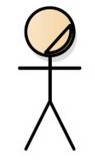
\includegraphics[height=3cm]{Data/actors.png}
      \end{figure}
      \end{column}

  \begin{column}{0.69\textwidth}
    \begin{itemize}
      \item Geographical Information System (GIS)
      \item Grid Operation Scheduler (GOS)
      \item Weather Forecast (WF)
      \item Reserve Aggregator (RA)
      \item Energy Forecaster (EF)
      \item Transmission System Operator (TSO)
      \item Distribution System Operator (DSO)
      \item Transmission Management System (TMS)
      \item Distribution Management System (DMS)
    \end{itemize}
      \end{column}

    \end{columns}

  \end{frame}

  \begin{frame}{Business and function layer}


\begin{figure}[!htb]\centering
  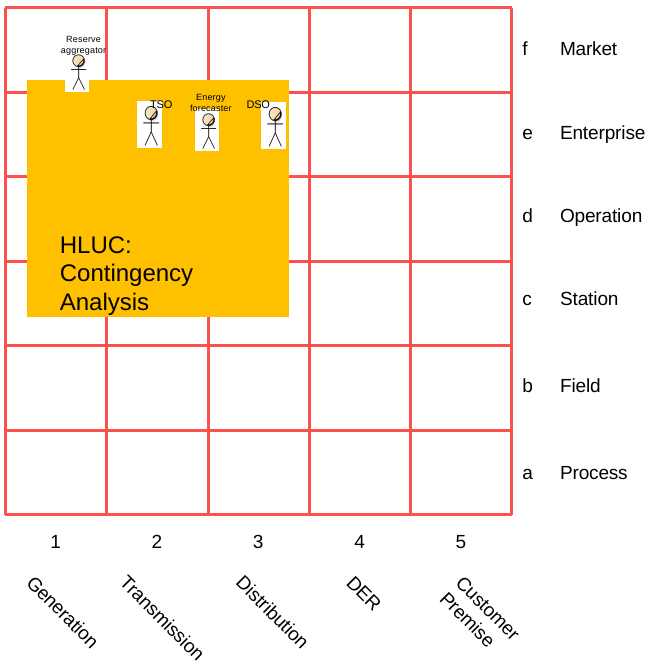
\includegraphics[width=6.0cm]{Data/business.png}
  \hspace{0.1cm}
  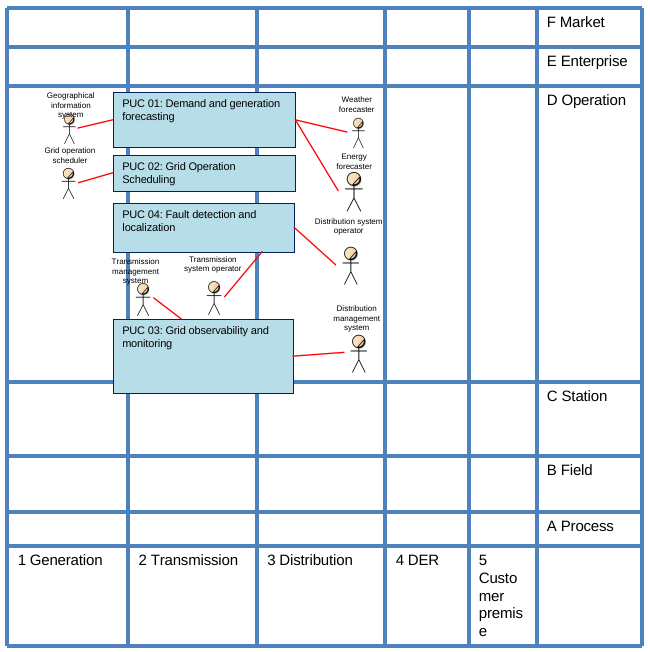
\includegraphics[width=6.0cm]{Data/function.png}
\caption{Business and function layer mapping}
\label{fig:functs}
\end{figure}





  \end{frame}


% -------------------------
\subsection{Context}
\begin{frame}{Context}
  \begin{itemize}
    \item Wind speeds exhibit unpredictable fluctuations.
    \item These variations in wind speed cause drastic changes in power:
  \end{itemize}

  \begin{equation}
    P_{wt} = \frac{1}{2}\rho AC_p v_w^3.
  \end{equation}

  Store the peaks of power and retrieve the energy once the wind speed diminishes.

  \vspace{0.5cm}

  \begin{figure}
    \centering
\begin{tikzpicture}
  \footnotesize
    \begin{axis}[xlabel={$t$ (s)}, ylabel={$v$ (m/s)}, grid=both, grid style={line width=.1pt, draw=gray!10}, major grid style={line width=.2pt,draw=gray!50}, xmin=0, ymin=8, xtick distance = 2, xmax=30, ytick distance = 1,  width=13.0cm, height=4cm, every plot/.append style={thick}, thick, grid=both, grid style={line width=.4pt, draw=gray!10}, major grid style={line width=.8pt,draw=gray!50}, legend style={at={(0.55,0.2)},anchor=south west}, /pgf/number format/.cd, 1000 sep={}]]
        % \addplot[color=black] table[col sep=comma, x=x, y=y] {Data/vw_profile1.csv};
        \addplot[color=black] table[col sep=comma, x=x, y=y] {Data/vw3.csv};
        % \addplot[color=black] table[col sep=comma, x=x, y=y] {Data/Tm2.csv};
\end{axis}
\end{tikzpicture}
\caption{Example of wind speed profile}
\end{figure}
\end{frame}


\subsection{Aim of the project}
\begin{frame}{Aim of the project}
  Goals:
  \begin{itemize}
    \item Minimize the fluctuations in the power exchanged with the grid.
    \item Ensure the supercapacitor operates inside the allowed limits.
    \item Quantify the results and compare them with other techniques.
  \end{itemize}

  Steps:
  \begin{enumerate}
    \item Model the back-to-back converter configuration of a wind turbine.
    \item Size the energy storage unit (supercapacitor).
    \item Model the control of a buck converter to integrate the supercapacitor.
    \item Test the full model in Matlab/Simulink for a realistic scenario.
  \end{enumerate}
\end{frame}


% ------------------
\section{Models}
\subsection{General scheme}
\begin{frame}{General scheme}

\begin{figure}
\centering
\begin{circuitikz}[>=latex', scale=0.7, transform shape,][american]
\tikzstyle{block} = [draw, rectangle, minimum height=1cm, minimum width=2cm]
\ctikzset{tripoles/mos style/arrows}
\ctikzset{tripoles/pmos style/nocircle}
\tikzset{sdcdc/.style={twoportsplit, t1={$=$}, t2={$=$}}}

\draw (1.5,-7.0) to[short] (3.5,-7.0);
\draw (1.5,-7.0) to[short] (1.5,-10.0);
\draw (1.5,-10.0) to[short] (3.5,-10.0);
\draw (8.5,-7.0) to[short] (8.5,-10.0);
\draw (8.5,-7.0) to[short] (10.5,-7.0);
\draw (8.5,-10.0) to[short] (10.5,-10.0);
\draw (4.0,-7.0) to[short] (4.0,-10.0);
\draw (3.5,-10.0) to[short] (4.0,-10.0);
\draw (3.5,-7.0) to[short] (4.0,-7.0);
\draw (10.5,-7.0) to[short] (11.0,-7.0);
\draw (10.5,-10.0) to[short] (11.0,-10.0);
\draw (11.0,-10.0) to[short] (11.0,-7.0);
\draw (3.0,-8.5) node[nmos](Q5){Q1};\draw (Q5.D) to[short] (3.0,-7.5);
\draw (Q5.S) to[short] (3.0,-9.5);
\draw (Q5.G) to[short] (2.0,-8.5);
\draw (10.0,-8.5) node[nmos](Q6){Q2};\draw (Q6.D) to[short] (10.0,-7.5);
\draw (Q6.S) to[short] (10.0,-9.5);
\draw (Q6.G) to[short] (9.0,-8.5);
\draw (4.0,-7.5) to[short] (8.5,-7.5);
\draw (4.0,-9.5) to[short] (8.5,-9.5);
\draw (5.0,-7.5) to[C] (5.0,-9.5);
\node[] at (5.5, -8.1) {$C_{dc}$};

\draw (6.0,-7.5) to[short, *-] (6.0,-11.2);
\draw (5.0,-9.5) to[short, *-] (5.0,-11.8);
\draw (5.0,-11.8) to[short, -*] (6.5,-11.8);
\draw (6.0,-11.2) to[short, -*] (6.5,-11.2);

% add dc/dc converter!!!
\draw (6.5,-11.5) to[sdcdc] (7.5,-11.5);
% \draw (0,0) to [twoportsplit, t1={$=$}, t2={$=$}] ++(3,0);
% \draw (0,0) to [twoportsplit] ++(3,0);

\draw (7.5,-11.2) -- (8.1, -11.2);
\draw (7.5,-11.8) -- (8.1, -11.8);
\draw (8.1, -11.0) -- (8.1,-12);
\draw (8.5, -11.0) -- (8.5,-12);
\draw (8.1,-11.0) -- (8.5,-11.0);
\draw (8.1,-12.0) -- (8.5,-12.0);
\node[] at (8.3, -11.2) {$+$};
\node[] at (8.3, -11.8) {$-$};
% \draw[in=170, out=190] (8.0,-11.2) to [open, v^=$v_c$] (8.0,-11.8);
\draw[->] plot [smooth] coordinates {(7.9, -11.25) (7.95, -11.5) (7.9,-11.8)};
\node[] at (7.7,-11.5) {$v_c$};

\draw[->] plot [smooth] coordinates {(7.5, -7.55) (7.6, -8.5) (7.5,-9.45)};
\node[] at (7.3,-8.5) {$V_{dc}$};

\draw (7.0,-13.0) node[block, scale=1] (block5) {$SOC$ control};
\draw [->] (7.0,-12.5) -- (7.0,-12.0);
\draw [->] (5.35,-13.0) -- (5.85,-13.0);
\draw [->] (7.0,-14.0) -- (7.0,-13.5);

\node[] at (4.9,-13.0) {$SOC^*$};
\node[] at (7.0,-14.2) {$v_{c}$};
\node[] at (6.7,-12.3) {$\alpha$};

\draw (2.5,-11.5) node[block, scale=1] (block6) {VSC turbine};
\draw (10.0,-11.5) node[block, scale=1] (block7) {VSC grid};
\draw [->] (10.0,-11.0) -- (10.0,-10.0);
\draw [->] (2.5,-11.0) -- (2.5,-10.0);
\node[] at (2.0, -10.5) {$v^*_{s,abc}$};


\draw (11.0,-8.5) to[L,l=$L_f$] (13.0,-8.5);
\draw[line width=0.05cm] (14.0,-8.0) to[short] (14.0,-9.0);
\draw (13.0,-8.5) to[short] (14.0,-8.5);
\draw [->] (11.5,-11.3) -- (11.0,-11.3);
\draw [->] (11.5,-11.7) -- (11.0,-11.7);
\draw [->] (9.3,-12.5) -- (9.3,-12.0);
\draw [->] (10.0,-12.5) -- (10.0,-12.0);
\draw [->] (10.7,-12.5) -- (10.7,-12.0);

\node[] at (9.3, -12.8) {$V^*_{dc}$};
\node[] at (10.0,-12.8) {$Q^*_g$};
\node[] at (10.7, -12.8) {$V_{dc}$};
\node[] at (12,-11.3) {$v_{g,abc}$};
\node[] at (12,-11.7) {$i_{g,abc}$};

\draw[->] (13.2, -8.5) to [short, o-] (13.2, -8.0);
\draw[->] (12.8, -8.7) to [short] (13.3, -8.7);
\node[] at (13.2,-9.0) {$i_{g,abc}$};
\node[] at (13.2,-7.8) {$v_{g,abc}$};

\node[] at (9.5,-10.5) {$v^*_{c,abc}$};
\node[] at (14.5,-8.5) {Grid};

\node[] at (0.4,-11.7) {$i_{s,abc}$};
\node[] at (0.4,-11.3) {$v_{s,abc}$};

\draw [->] (3.0,-12.5) -- (3.0,-12.0);
\draw (-0.5,-13.5) node[block, scale=1] (block11) {MPPT};
\draw [->] (-0.5,-12.5) -- (-0.5,-13.0);
\draw [->] (-2.0,-13.5) -- (-1.5,-13.5);
\draw [->] (-0.5,-14.5) -- (-0.5,-14.0);


\node[] at (-0.5,-12.3) {$v_w$};
\node[] at (-2.4,-13.5) {$\omega_m$};
\node[] at (-0.5,-14.7) {$\theta_p$};


\node[] at (2.8,-6.7) {VSC1};
\node[] at (9.8,-6.7) {VSC2};

\draw (0.5,-13.5) -- (1.0,-13.5);
\draw (1.0,-13.5) -- (2.0, -13.5);
\draw[->] (2.0, -13.5) -- (2,-12.0);
\node[] at (1.7,-12.8) {$T^*$};
\node[] at (3,-12.8) {$Q_s^*$};

% \draw [->] (1.0,-11.3) -- (1.50,-11.3);
\draw [->] (0.9,-11.3) -- (1.4,-11.3);
\draw [->] (0.9,-11.7) -- (1.4,-11.7);


% pmsg
\draw (-0.5,-8.5) circle(0.8cm);
\draw (-0.5,-8.5) circle(0.6cm);
\draw[fill=black] (-0.5,-8.5) circle(0.1cm);
\draw[line width=0.07cm] (-0.5, -8.5) -- (-1.75,-8.5); 
\draw (-1.75,-8.6) -- (-2, -8.6);
\draw (-1.75,-8.4) -- (-2, -8.4);
\draw (-1.75, -8.6) -- (-1.75, -8.4);
\draw (-2,-8.5) -- (-2,-8.3);
\draw (-2,-8.5) -- (-2,-8.7);
\draw (-2,-8.7) -- (-2.25, -8.7);
\draw (-2,-8.3) -- (-2.25, -8.3);
\draw (-2,-10) -- (-2,-7.0);
\draw (0.3, -8.5) -- (1.5,-8.5);
\draw[->] (-1.6,-8.5) to [short, o-] (-1.6, -9.5);
\node[] at (-1.6,-9.7) {$\omega_m$};

\draw[->] (1.0,-8.5) to [short, o-] (1.0, -8.0);
\draw[->] (0.6,-8.7) to [short] (1.1, -8.7);
\node[] at (0.8,-9.0) {$i_{s,abc}$};
\node[] at (1.0,-7.8) {$v_{s,abc}$};

\draw plot [smooth] coordinates {(-2,-10) (-2.1,-9.4) (-2.2,-9) (-2.18,-8.7)};
\draw plot [smooth] coordinates {(-2,-7) (-2.1,-7.6) (-2.2,-8) (-2.18,-8.3)};
\draw plot [smooth] coordinates {(-2.25,-8.3) (-2.35,-8.35) (-2.5,-8.5) (-2.35,-8.65) (-2.25,-8.7)};

\draw (-2.2,-8.9) -- (-2,-8.9);
\draw (-2.2,-8.1) -- (-2,-8.1);

\draw[->] (-2.8, -9.5) -- (-2.3, -9.5);
\draw[->] (-2.8, -7.5) -- (-2.3, -7.5);

\node[] at (-2.8,-9.3) {$v_{w}$};
\node[] at (-1.65,-7.7) {$\theta_{p}$};

\end{circuitikz}
\caption{Scheme of the full system with the turbine, the converters, and the energy storage unit}
\label{fig:full}
\end{figure}

\end{frame}


\subsection{MPPT}
\begin{frame}{Maximum power point tracking}
  The machine-side converter has to be controlled so as to extract the maximum power from the wind. 

\begin{figure}
\centering
\begin{circuitikz}[>=latex', scale=0.7, transform shape][american]
\tikzstyle{block} = [draw, rectangle, minimum height=1cm, minimum width=2cm]
\draw (0.5,-1.5) node[block, scale=1] (block1) {$\frac{1}{2}\rho A v_{w}^3 C_p$};
\draw [->] (-1.0,-1.5) -- (-0.5,-1.5);
\draw (3.0,-1.5) node[mixer, scale=1] (mixer1) {};
\draw [->] (1.5,-1.5) -- (2.5,-1.5);
\draw [->] (3.0,-2.5) -- (3.0,-2.0);
\draw (5.0,-1.5) node[mixer, scale=1] (mixer2) {};
\draw [->] (3.5,-1.5) -- (4.5,-1.5);
\draw [->] (5.0,-2.5) -- (5.0,-2.0);
\draw (7.0,-1.5) node[block, scale=1] (block2) {$\frac{1}{s}\frac{1}{J_{eq}}$};
\draw [->] (5.5,-1.5) -- (6.0,-1.5);
\draw (9.5,-1.5) node[mixer, scale=1] (mixer3) {};
\draw (8.0,-1.5) to[short] (8.5,-1.5);
\draw (8.5,-1.5) to[short] (8.5,-0.5);
\draw (8.5,-0.5) to[short] (9.5,-0.5);
\draw (8.5,-1.5) to[short] (8.5,-2.5);
\draw (8.5,-2.5) to[short] (9.5,-2.5);
\draw [->] (9.5,-2.5) -- (9.5,-2.0);
\draw [->] (9.5,-0.5) -- (9.5,-1.0);
\draw (11.5,-1.5) node[block, scale=1] (block4) {$K_{cp}$};
\draw [->] (10.0,-1.5) -- (10.5,-1.5);
\draw [->] (12.5,-1.5) -- (13.0,-1.5);
\draw (-1.0,-1.8) node[] {$v_{w}$};
\draw (-1.0,-1.2) node[] {$\theta_p$};
\draw (3.0,-2.8) node[] {$\omega_m$};
\draw (5.0,-2.8) node[] {$T_e$};
\draw (2.0,-1.8) node[] {$P_{wt}$};
\draw (4.0,-1.8) node[] {$T_m$};
\draw (9.9,-0.6) node[] {$\omega_m$};
\draw (9.9,-2.4) node[] {$\omega_m$};
\draw (13.0,-1.8) node[] {$T_{e,opt}$};

\draw (2.70,-1.5) node[] {x};
\draw (3.0,-1.8) node[] {$\div$};

\draw (4.70,-1.5) node[] {$+$};
\draw (5.00,-1.8) node[] {$-$};

\draw (9.5,-1.2) node[] {x};
\draw (9.5,-1.8) node[] {x};

\end{circuitikz}
\caption{Block diagram of the MPPT}
\label{fig:mppt}
\end{figure}

The key part is the quadratic relationship between speed and torque:
\begin{equation}
   K_{cp} = \frac{1}{2}\rho A \left(\frac{D}{2}\right)^3 \left(\frac{c_1}{c_2^2c_7^4}(c_2 + c_6 c_7)^3 e^{-(c_2+c_6c_7)/c_2}\right).
\end{equation}


\end{frame}


\subsection{Machine-side converter}
\begin{frame}{Machine-side converter}
  Two references are received: reactive power and optimal torque.

\begin{columns}
\begin{column}{0.5\textwidth}
  \parbox{1\textwidth}{

\begin{figure}
\centering
\begin{circuitikz}[>=latex', scale=0.7, transform shape][american]
\tikzstyle{block} = [draw, rectangle, minimum height=1cm, minimum width=2cm]
\draw (2.5,-0.0) node[mixer, scale=1] (mixer1) {};
\draw [->] (1.5,-0.0) -- (2.0,-0.0);
\draw [->] (2.5,-1.0) -- (2.5,-0.5);
\draw (5.0,-0.0) node[block, scale=1] (block1) {$k_{q,p} + \frac{k_{q,i}}{s}$};
\draw (8.0,-0.0) node[block, scale=1] (block2) {$\frac{2}{3}\hat{V}$};
\draw [->] (6.0,-0.0) -- (7.0,-0.0);
\draw [->] (3.0,-0.0) -- (4.0,-0.0);
\draw [->] (9.0,-0.0) -- (9.5,-0.0);
\draw (8.0,-2.0) node[block, scale=1] (block4) {$\frac{2}{3p_p\psi}$};
\draw [->] (9.0,-2.0) -- (9.5,-2.0);
\draw [->] (6.5,-2.0) -- (7.0,-2.0);
\draw (1.5,-0.3) node[] {$Q^*$};
\draw (2.5,-1.3) node[] {$Q$};
\draw (9.5,-0.3) node[] {$i^*_d$};
\draw (9.5,-2.3) node[] {$i^*_q$};
\draw (6.5,-2.3) node[] {$T_{e,opt}$};
\draw (2.2,-0.0) node[] {$+$};
\draw (2.5,-0.3) node[] {$-$};
\end{circuitikz}
\caption{Reactive power control and current references calculation}
\label{fig:Qmach}
\end{figure}


}
\end{column}

\begin{column}{0.5\textwidth}
  \parbox{1\textwidth}{


\begin{figure}[!htb]
\centering
\begin{circuitikz}[>=latex', scale=0.7, transform shape][american]
\tikzstyle{block} = [draw, rectangle, minimum height=1cm, minimum width=2cm]
\draw (2.0,-0.0) node[mixer, scale=1] (mixer1) {};
\draw (4.5,-0.0) node[block, scale=1] (block1) {$k_{c,p} + \frac{k_{c,i}}{s}$};
\draw (7.0,-0.0) node[mixer, scale=1] (mixer5) {};
\draw (4.5,-4.5) node[block, scale=1] (block6) {$k_{c,p} + \frac{k_{c,i}}{s}$};
\draw (7.0,-4.5) node[mixer, scale=1] (mixer7) {};
\draw (2.0,-4.5) node[mixer, scale=1] (mixer8) {};
\draw [->] (1.0,-0.0) -- (1.5,-0.0);
\draw [->] (1.0,-4.5) -- (1.5,-4.5);
% \draw [->] (7.0,-5.5) -- (7.0,-5.0);
\draw [->] (7.0,1.0) -- (7.0,0.5);
\draw [->] (7.5,-0.0) -- (8.0,-0.0);
\draw [->] (7.5,-4.5) -- (8.0,-4.5);
\draw [->] (7.0,-2.0) -- (7.0,-0.5);
\draw [->] (7.0,-2.5) -- (7.0,-4.0);
\draw (5.0,-3.0) to[short] (7.0,-2.0);
\draw (5.0,-1.5) to[short] (7.0,-2.5);
\draw [->] (5.5,-0.0) -- (6.5,-0.0);
\draw [->] (5.5,-4.5) -- (6.5,-4.5);
\draw [->] (2.5,-4.5) -- (3.5,-4.5);
\draw [->] (2.5,-0.0) -- (3.5,-0.0);
\draw (4.5,-3.0) node[mixer, scale=1] (mixer10) {};
\draw (4.5,-1.5) node[mixer, scale=1] (mixer11) {};
\draw (2.5,-2.25) node[block, scale=1] (block8) {$L_{qd}$};
\draw [->] (4.5,-2.5) -- (4.5,-2.0);
\draw [->] (4.5,-2.0) -- (4.5,-2.5);
\draw (3.5,-2.25) to[short] (4.5,-2.25);
\draw (1.0,-3.75) to[short] (4.5,-3.75);
\draw (1.0,-0.75) to[short] (4.5,-0.75);

\draw [->] (4.5,-0.75) -- (4.5,-1.0);
\draw [->] (4.5,-3.75) -- (4.5,-3.5);

\draw [->] (2.0,-0.75) -- (2.0,-0.5);
\draw [->] (2.0,-3.75) -- (2.0,-4.0);
\draw (1.0,0.3) node[] {$i_q^*$};
\draw (1.0,-1.0) node[] {$i_q$};
\draw (1.0,-3.5) node[] {$i_d$};
\draw (1.0,-4.8) node[] {$i_d^*$};
% \draw (7.0,1.2) node[] {$\omega_m p_p \psi$};
\draw (7.7,0.9) node[] {$\omega_m p_p \psi$};
\draw (8.0,-0.3) node[] {$v_q$};
\draw (8.0,-4.8) node[] {$v_d$};
\draw [->] (1.0,-2.25) -- (1.5,-2.25);
\draw (1.0,-2.5) node[] {$\omega_mp_p$};

\draw (4.20,-3) node[] {x};
\draw (4.20,-1.5) node[] {x};

\draw (4.50,-2.7) node[] {x};
\draw (4.50,-1.8) node[] {x};

\draw (2.0,-0.3) node[] {$-$};
\draw (2.0,-4.2) node[] {$-$};

\draw (1.7,-0.0) node[] {$+$};
\draw (1.7,-4.5) node[] {$+$};

\draw (7.0,-4.2) node[] {$-$};
\draw (6.7,-4.5) node[] {$+$};

\draw (7.0,-0.3) node[] {$+$};
\draw (7.0,0.3) node[] {$+$};
\draw (6.7,-0.0) node[] {$+$};

\end{circuitikz}
\caption{Inner current control loop}
\label{fig:currentloop}
\end{figure}

}

\end{column}
\end{columns}

With the inner current control loop, the current references are transformed into the $qd$ voltages to synthetize.

\end{frame}


\subsection{Grid-side converter}
\begin{frame}{Grid-side converter}
Two references are received: the DC bus voltage and the reactive power to exchange with the grid.

\begin{figure}
\centering
\begin{circuitikz}[>=latex', scale=0.7, transform shape][american]
\tikzstyle{block} = [draw, rectangle, minimum height=1cm, minimum width=2cm]
\draw (3.5,-0.0) node[block, scale=1] (block1) {$k_{v,p} + \frac{k_{v,i}}{s}$};
\draw (6.0,-0.0) node[mixer, scale=1] (mixer2) {};
\draw (1.0,-0.0) node[mixer, scale=1] (mixer3) {};
\draw (8.5,-0.0) node[block, scale=1] (block2) {$\frac{2}{3}\frac{V^*_{dc}}{\hat{V}}$};
\draw [->] (0.0,-0.0) -- (0.5,-0.0);
\draw [->] (1.5,-0.0) -- (2.5,-0.0);
\draw [->] (4.5,-0.0) -- (5.5,-0.0);
\draw [->] (6.0,-1.0) -- (6.0,-0.5);
\draw [->] (1.0,-1.0) -- (1.0,-0.5);
\draw [->] (6.5,-0.0) -- (7.5,-0.0);
\draw [->] (9.5,-0.0) -- (10.0,-0.0);
\draw (8.5,-2.5) node[block, scale=1] (block3) {$k_{q,p} + \frac{k_{q,i}}{s}$};
\draw (5.5,-2.5) node[block, scale=1] (block4) {$\frac{2}{3}\hat{V}$};
\draw (3.0,-2.5) node[mixer, scale=1] (mixer4) {};
\draw [->] (2.0,-2.5) -- (2.5,-2.5);
\draw [->] (3.0,-3.5) -- (3.0,-3.0);
\draw [->] (3.5,-2.5) -- (4.5,-2.5);
\draw [->] (6.5,-2.5) -- (7.5,-2.5);
\draw [->] (9.5,-2.5) -- (10.0,-2.5);
\draw (0.0,-0.3) node[] {$V^*_{dc}$};
\draw (1.0,-1.3) node[] {$V_{dc}$};
\draw (2.0,-2.8) node[] {$Q^*$};
\draw (3.0,-3.8) node[] {$Q$};
\draw (6.0,-1.3) node[] {$I_{dc}$};
\draw (10.0,-2.8) node[] {$i^*_q$};
\draw (10.0,-0.3) node[] {$i^*_d$};

\draw (0.7,-0.0) node[] {$+$};
\draw (1.0,-0.3) node[] {$-$};

\draw (2.7,-2.5) node[] {$+$};
\draw (3.0,-2.8) node[] {$-$};

\draw (5.7,-0.0) node[] {$+$};
\draw (6.0,-0.3) node[] {$-$};


\end{circuitikz}
\caption{Reactive power control and DC voltage control loop}
\label{fig:QVgrid}
\end{figure}

Just like before, an inner current control loop is also present. 

\end{frame}

\subsection{Supercapacitor control}
\begin{frame}{Buck converter}
  Responsible for controlling the charge and discharge processes of the supercapacitor.

\begin{figure}
\centering
\begin{circuitikz}[>=latex', scale=0.7, transform shape][american]
\tikzstyle{block} = [draw, rectangle, minimum height=1cm, minimum width=2cm]
\ctikzset{tripoles/mos style/arrows}
\ctikzset{tripoles/pmos style/nocircle}
\ctikzset{diodes/scale=0.4}
\ctikzset{resistors/scale=0.75}

% boxes
\node[draw, thick, minimum width=4.3cm, minimum height=3.25cm, fill=gray!10, rounded corners=0.2cm, dashed] at (11.4, -8.25){};
\node[] at (11.4, -6.4) {Supercapacitor};
\node[draw, thick, minimum width=4cm, minimum height=4.75cm, fill=gray!10, rounded corners=0.2cm, dashed] at (6.4, -7.5){};
\node[] at (6.4, -4.9) {DC/DC converter};
\node[draw, thick, minimum width=2cm, minimum height=4.75cm, fill=gray!10, rounded corners=0.2cm, dashed] at (2.7, -7.5){};
\node[] at (2.7, -4.9) {DC bus};

\draw (6.5,-7.5) to[L,l=$L$] (8.5,-7.5);
\draw (6.0,-7.5) to [short] (6.5, -7.5);
\draw (8.5,-7.5) to[short, i=$i_{sc}$] (9.0,-7.5);
\draw (9.0,-7.5) to[R,l=$R_s$] (11.0,-7.5);
\draw (11.0,-7.5) to[R,l_=$R_p$] (11.0,-9.5);
\draw (12.5,-7.5) to[C,l=$C$, v_=$V_{c}$] (12.5,-9.5);
\draw (11.0,-7.5) to[short] (12.5,-7.5);
\draw (11.0,-9.5) to[short] (12.5,-9.5);
\draw (11.0,-9.5) to[short] (6.0,-9.5);
\draw (6.0,-8.5) node[nigbt](Q3){};
\draw (5.0,-8.2) node[]{Q2};
\draw (Q3.C) to[short] (6.0,-7.5);
\draw (Q3.E) to[short] (6.0,-9.5);
\draw (Q3.B) to[short] (5.0,-8.5);

\draw (6.35,-9.0) to[D] (6.35,-8.0);
\draw (6.0,-8.0) to[short] (6.35,-8.0);
\draw (6.35,-9.0) to[short] (6.0,-9.0);
\draw (6.0,-6.5) node[nigbt](Q4){};
\draw (5.0,-6.2) node[]{Q1};
\draw (Q4.C) to[short] (6.0,-5.5);
\draw (Q4.E) to[short] (6.0,-7.5);
\draw (Q4.B) to[short] (5.0,-6.5);
\draw (6.35,-7.0) to[D] (6.35,-6.0);
\draw (6.35,-6.0) to[short] (6.0,-6.0);
\draw (6.35,-7.0) to[short] (6.0,-7.0);
\draw (6.0,-5.5) to[short] (2.5,-5.5);
\draw (6.0,-9.5) to[short] (2.5,-9.5);
\draw (3.0,-5.5) to[C,l_=$C_{dc}$] (3.0,-9.5);

\end{circuitikz}
\caption{DC/DC buck converter with the supercapacitor}
\label{fig:dcdc}
\end{figure}
Switches Q1 and Q2 are turned on and off according to the desired duty cycle $D$.


\end{frame}

\begin{frame}{Supercapacitor control}

  \begin{columns}

\begin{column}{0.6\textwidth}
  \parbox{1\textwidth}{

\begin{figure}
   \centering
   \begin{circuitikz}[>=latex', scale=0.7, transform shape][american]
   \tikzstyle{block} = [draw, rectangle, minimum height=1cm, minimum width=2cm]
   \draw (2.0,-0.0) node[mixer, scale=1] (mixer1) {};
   \draw [->] (1.0,-0.0) -- (1.5,-0.0);
   \draw [->] (2.0,-1.0) -- (2.0,-0.5);
   \draw (4.5,-0.0) node[block, scale=1] (block1) {$k_{s,p} + \frac{k_{s,i}}{s}$};
   \draw (7.0,-0.0) node[mixer, scale=1] (mixer2) {};
   \draw [->] (5.5,-0.0) -- (6.5,-0.0);
   \draw [->] (7.0,-1.0) -- (7.0,-0.5);
   \draw [->] (2.5,-0.0) -- (3.5,-0.0);
   \draw [->] (7.5,-0.0) -- (8.5,-0.0);
   \draw (9.5,-0.0) node[block, scale=1] (block2) {$k_{ic,p} + \frac{k_{ic,i}}{s}$};
   \draw [->] (10.5,-0.0) -- (11.0,-0.0);
   \draw (1.0,-0.3) node[] {$SOC^*$};
   \draw (2.0,-1.3) node[] {$SOC$};
   \draw (7.0,-1.3) node[] {$i_{sc}$};
   \draw (11.0,-0.3) node[] {$D$};
   \draw (6.0,-0.3) node[] {$i^*_{sc}$};

\draw (1.7,-0.00) node[] {$+$};
\draw (2.0,-0.30) node[] {$-$};

\draw (6.7,-0.00) node[] {$+$};
\draw (7.0,-0.30) node[] {$-$};

   \end{circuitikz}
   \caption{Control diagram of the SOC of the supercapacitor}
   \label{fig:Dcycle}
\end{figure}

\begin{figure}[!htb]
   \centering
   \begin{circuitikz}[>=latex', scale=0.7, transform shape][american]
   \tikzstyle{block} = [draw, rectangle, minimum height=1cm, minimum width=2cm]
   \draw (5.0,0.5) node[block, scale=1] (block3) {$H(s)$};
   \draw (5.0,-1.5) node[block, scale=1] (block4) {$G(s)$};
   \draw (8.0,-1.5) node[block, scale=1] (block5) {$k_{low}$};
   \draw (8.0,0.5) node[block, scale=1] (block6) {$k_{high}$};
   \draw (10.5,-0.5) node[mixer, scale=1] (mixer3) {};
   \draw [->] (11.0,-0.5) -- (11.5,-0.5);
   \draw (9.0,0.5) to[short] (10.5,0.5);
   \draw (9.0,-1.5) to[short] (10.5,-1.5);
   \draw [->] (10.5,-1.5) -- (10.5,-1.0);
   \draw [->] (10.5,0.5) -- (10.5,-0.0);
   \draw [->] (6.0,0.5) -- (7.0,0.5);
   \draw [->] (6.0,-1.5) -- (7.0,-1.5);
   \draw (4.0,0.5) to[short] (3.5,0.5);
   \draw (3.5,0.5) to[short] (3.5,-1.5);
   \draw (3.5,-1.5) to[short] (4.0,-1.5);
   \draw [->] (3.0,-0.5) -- (3.5,-0.5);
   \draw (11.5,-0.8) node[] {$SOC^*$};
   \draw (3.0,-0.8) node[] {$v_w$};

\draw (10.5,-0.20) node[] {$+$};
\draw (10.5,-0.80) node[] {$+$};

   \end{circuitikz}
   \caption{Calculation of the reference of the SOC}
   \label{fig:socref}
   \end{figure}




}
\end{column}


% bodes
\begin{column}{0.4\textwidth}
  \parbox{1\textwidth}{

\begin{figure}[!htb]
  \footnotesize

   \centering
\begin{tikzpicture}
    \begin{axis}[xmode=log, xlabel={Frequency (Hz)}, ylabel={Magnitude (dB)}, grid=both, grid style={line width=.1pt, draw=gray!10}, major grid style={line width=.2pt,draw=gray!50}, ytick distance = 20,  width=5.0cm, height=3.5cm, every plot/.append style={very thick},  very thick, grid=both, grid style={line width=.4pt, draw=gray!30}, major grid style={line width=.8pt,draw=gray!50}, legend style={at={(1.03,0.04)},anchor=south west}]
        \addplot[color=black] table[col sep=comma, x=x, y=y] {Data/Calculations/mag_low.csv};
\end{axis}
\end{tikzpicture}
\vspace{0.1cm}
\begin{tikzpicture}
    \begin{axis}[xmode=log, xlabel={Frequency (Hz)}, ylabel={Magnitude (dB)}, grid=both, grid style={line width=.1pt, draw=gray!10}, major grid style={line width=.2pt,draw=gray!50}, ytick distance = 20,  width=5.0cm, height=3.5cm, every plot/.append style={very thick},  very thick, grid=both, grid style={line width=.4pt, draw=gray!30}, major grid style={line width=.8pt,draw=gray!50}, legend style={at={(1.03,0.04)},anchor=south west}]
        \addplot[color=black] table[col sep=comma, x=x, y=y] {Data/Calculations/mag_high.csv};
\end{axis}
\end{tikzpicture}

\caption{Bode plot of $H(s)$ and $G(s)$}

    \label{fig:Gow}
\end{figure}



 }

 \end{column}
 \end{columns}

\end{frame}



% ------------------
\section{Sizing}
\subsection{Calculations}
\begin{frame}{Sizing calculations}
  The supercapacitor is sized based on a sinusoidal perturbation:

  \vspace{0.5cm}
\begin{figure}
  \centering
\incfig{supercap3}
\caption{Perturbation and SOC as a function of the voltage of the supercapacitor}
\label{fig:socc}
\end{figure}
\vspace{-0.2cm}
  \begin{equation}
    C = \frac{8 \frac{P_n}{\omega_c}}{V^2_{max} - V^2_{min}}.
  \end{equation}

\end{frame}

\subsection{Configuration}
\begin{frame}{Configuration}
  \begin{itemize}
    \item For the considered case study, $C=0.91$~F.
    \item Configuration of 4 parallel branches and about 1600 series cells. 
    \item In total, they occupy about 0.382~m$^3$ and last for 500000 cycles.
  \end{itemize}

  \begin{figure}
    \footnotesize
    \incfig{config_caps2}
    \caption{Chosen configuration of cells}
    \label{fig:cells}
  \end{figure}

\end{frame}


% ------------------
\section{Results}
\subsection{Indicators}
\begin{frame}{Indicators}
  Apart from qualitative observations, quantitative indicators are considered. Assessment based on:
\begin{itemize}
      \item Maximum variation in the output power:
    \end{itemize}
    \begin{equation}
      \Delta P = \max{(P)} - \min{(P)}.
    \end{equation}
  \begin{itemize}
    \item Roughness index:
  \end{itemize}
  \begin{equation}
    RI = \sum_{i=1}^{n-1}\left[ P(i+1) - P(i) \right]^2.
  \end{equation}
  \begin{itemize}
  \item Simple moving average:
  \end{itemize}
  \begin{equation}
    SMA_k = \frac{1}{k} \sum_{i=n-k-1}^n P(i).
  \end{equation}
    
\end{frame}

\subsection{Example}
\begin{frame}{Example in a two-bus system}
The supercapacitor mitigates the fluctuations to obtain a smoother power profile.
  \begin{figure}
    \centering
\begin{tikzpicture}
  \footnotesize
    \begin{axis}[xlabel={$t$ (s)}, ylabel={$P$ (MW)}, grid=both, grid style={line width=.1pt, draw=gray!10}, major grid style={line width=.2pt,draw=gray!50}, xmin=4, xtick distance = 1, xmax=11.5, ytick distance = 0.2,  width=13.0cm, height=4cm, every plot/.append style={thick}, thick, grid=both, grid style={line width=.4pt, draw=gray!10}, major grid style={line width=.8pt,draw=gray!50}, legend style={at={(0.75,0.1)},anchor=south west}, /pgf/number format/.cd, 1000 sep={}]]
        % \addplot[color=black] table[col sep=comma, x=x, y=y] {Data/vw_profile1.csv};
        \addplot[color=black] table[col sep=comma, x=x, y=y] {Data/Pmech.csv};
        \addplot[color=blue] table[col sep=comma, x=x, y=y] {Data/Pgrid.csv};
        % \addplot[color=black] table[col sep=comma, x=x, y=y] {Data/Tm2.csv};
        \legend{$P_{mech}$, $P_{grid}$}
\end{axis}
\end{tikzpicture}
\caption{Mechanical power and active power exchanged with the grid}
\end{figure}

\begin{table}
  \begin{tabular}{ccc}
    \hline
    \textbf{Indicator} & $\bm{P_{mech}}$ & $\bm{P_{grid}}$ \\
    \hline
    $\Delta P$ (MW) & 0.531 & 0.439 \\
    $RI$ (MW$^2$) & 0.066 & 0.003 \\
    \hline
  \end{tabular}
    \caption{Numerical indicators results}
\end{table}

\end{frame}


% ------------------
\section{Conclusions}
\begin{frame}{Conclusions}
  \begin{itemize}
    \item The combination of type-IV wind turbines with an energy storage device offers great controllability.
      \item The supercapacitor manages to reduce the fluctuations in power.
        \item It was preferable to prioritize the low frequencies. However, other control strategies may be equally convenient, if not more.
  \end{itemize}
\end{frame}


% ------------------
\section{Bibliography}
\begin{frame}{Bibliography}
  \tiny
  \justifying
\begin{columns}
\begin{column}{0.5\textwidth}
  \parbox{1\textwidth}{
  1. F. Blaabjerg, F. Iov, R. Teodorescu, and Z. Chen, “Power electronics in renewable energy systems,” in 2006 12th International Power Electronics and Motion Control Conference, IEEE, 2006, pp. 1–17.
\vspace{0.1cm}

  2. H. Abu-Rub, M. Malinowski, and K. Al-Haddad, Power electronics for renewable energy systems, transportation and industrial applications. John Wiley \& Sons, 2014. 
\vspace{0.1cm}

  3. M.-H. Ryu, H.-S. Kim, J.-W. Baek, H.-G. Kim, and J.-H. Jung, “Effective test bed of 380-v dc distribution system using isolated power converters,” IEEE transactions on industrial electronics, vol. 62, no. 7, pp. 4525–4536, 2015.
  \vspace{0.1cm}

  4. IRENA, “Renewable capacity statistics 2021,” Abu Dabi, United Emirate States, Annual report, 2021.
  \vspace{0.1cm}

  5. F. Blaabjerg, M. Liserre, and K. Ma, “Power electronics converters for wind turbine systems,” IEEE Transactions on industry applications, vol. 48, no. 2, pp. 708–719, 2011.
  \vspace{0.1cm}

  6. O. Tremblay, R. Gagnon, and M. Fecteau, “Real-time simulation of a fully detailed type-iv wind turbine,” submitted to IPST, vol. 13, pp. 18–20, 2013.
  \vspace{0.1cm}

  7. N. Espinoza, M. Bongiorno, and O. Carlson, “Frequency characterization of type-iv wind turbine systems,” in 2016 IEEE Energy Conversion Congress and Exposition (ECCE), IEEE, 2016, pp. 1–8.
  \vspace{0.1cm}

  8. G. He, Q. Chen, C. Kang, Q. Xia, and K. Poolla, “Cooperation of wind power and battery storage to provide frequency regulation in power markets,” IEEE Transactions on Power Systems, vol. 32, no. 5, pp. 3559–3568, 2016.
  \vspace{0.1cm}

  9. G. Mandic, A. Nasiri, E. Ghotbi, and E. Muljadi, “Lithium-ion capacitor energy storage integrated with variable speed wind turbines for power smoothing,” IEEE Journal of emerging and selected topics in power electronics, vol. 1, no. 4, pp. 287–295, 2013.
  \vspace{0.1cm}
}
\end{column}

\begin{column}{0.5\textwidth}
  \parbox{1\textwidth}{
  10. W. C. de Carvalho, R. P. Bataglioli, R. A. Fernandes, and D. V. Coury, “Fuzzy-based approach for power smoothing of a full-converter wind turbine generator using a supercapacitor energy storage,” Electric Power Systems Research, vol. 184, p. 106 287, 2020.
  \vspace{0.1cm}

  11. P. Garasi, M. Watanabe, and Y. Mitani, “Power smoothing of wind turbine generator using fuzzy-pi pitch angle controller,” in 2014 Australasian Universities Power Engineering Conference (AUPEC), IEEE, 2014, pp. 1–5.
  \vspace{0.1cm}

  12. O. P. Mahela and A. G. Shaik, “Comprehensive overview of grid interfaced wind energy generation systems,” Renewable and Sustainable Energy Reviews, vol. 57, pp. 260–281, 2016.
  \vspace{0.1cm}

  13. G. O. Suvire, M. G. Molina, and P. E. Mercado, “Improving the integration of wind power generation into ac microgrids using flywheel energy storage,” IEEE Transactions on smart grid, vol. 3, no. 4, pp. 1945–1954, 2012.
  \vspace{0.1cm}

  14. L. Qu and W. Qiao, “Constant power control of dfig wind turbines with supercapacitor energy storage,” IEEE Transactions on Industry Applications, vol. 47, no. 1, pp. 359–367, 2010.
  \vspace{0.1cm}

  15. A. K. Arani, H. Karami, G. Gharehpetian, and M. Hejazi, “Review of flywheel energy storage systems structures and applications in power systems and microgrids,” Renewable and Sustainable Energy Reviews, vol. 69, pp. 9–18, 2017.
  \vspace{0.1cm}

  16. C. Abbey and G. Joos, “Supercapacitor energy storage for wind energy applications,” IEEE transactions on Industry applications, vol. 43, no. 3, pp. 769–776, 2007.
  \vspace{0.1cm}

  17. M. Ammar and G. Joós, “A short-term energy storage system for voltage quality improvement in distributed wind power,” IEEE Transactions on Energy Conversion, vol. 29, no. 4, pp. 997–1007, 2014.
  \vspace{0.45cm}
}

\end{column}
\end{columns}

\end{frame}

\begin{frame}{Bibliography}
  \tiny
  \justifying
\begin{columns}
\begin{column}{0.5\textwidth}
  \parbox{1\textwidth}{
  18. J. P. Queralt and O. G. Bellmunt, “Control of voltage source converters for distributed generation in microgrids,” PhD thesis, Universitat Politècnica de Catalunya, 2015.
  \vspace{0.1cm}

  19. M. Raza and O. Gomis-Bellmunt, “Control system of voltage source converter to interconnect offshore ac hub with multiple onshore grids,” in 2015 International Conference on Renewable Energy Research and Applications (ICRERA), IEEE, 2015, pp. 677–682.
  \vspace{0.1cm}

  20. M. Ragheb, “Wind energy conversion theory, betz equation,” Wind Energie, 2014.
  \vspace{0.1cm}

  21. T. Ackermann, Wind power in power systems. John Wiley \& Sons, 2012.
  \vspace{0.1cm}

  22. F. Diaz-González, A. Sumper, O. Gomis-Bellmunt, and F. D. Bianchi, “Energy management of flywheel-based energy storage device for wind power smoothing,” Applied energy, vol. 110, pp. 207–219, 2013.
  \vspace{0.1cm}

  23. A. Junyent-Ferré, O. Gomis-Bellmunt, A. Sumper, M. Sala, and M. Mata, “Modeling and control of the doubly fed induction generator wind turbine,” Simulation Modelling Practice and Theory, vol. 18, no. 9, pp. 1365–1381, 2010.
  \vspace{0.1cm}

  24. T.-t. Liu, Y. Tan, G. Wu, and S.-m. Wang, “Simulation of pmsm vector control system based on matlab/simulink,” in 2009 international conference on measuring technology and mechatronics automation, IEEE, vol. 2, 2009, pp. 343–346.
  \vspace{0.1cm}

  25. H. Mahmood, D. Michaelson, and J. Jiang, “Reactive power sharing in islanded microgrids using adaptive voltage droop control,” IEEE Transactions on Smart Grid, vol. 6, no. 6, pp. 3052–3060, 2015.
  \vspace{0.95cm}

}
\end{column}

\begin{column}{0.5\textwidth}

\end{column}
\end{columns}

\end{frame}





% most slides about the converters control schemes
% a couple of slides on sizing
% quantification (definition of indicators)
% some results, even if simple, maybe only 1 slide, with indicators
% conclusions
% bibliography!! even if not cited, just put a list of papers that we have on the bibliography of the main report
